\documentclass[%
%%% PARA ESCOLHER O ESTILO TIRE O SIMBOLO %(COMENTÁRIO)
%SemVinculoColorido,
SemFormatacaoCapitulo,
SemFolhaAprovacao,
%SemImagens,
%CitacaoNumerica, %% o padrão é citação tipo autor-data
%PublicacaoDissOuTese, %% (é também o "default") com ficha catal. e folha de aprovação em branco. Caso tenha lista de símbolos e lista de siglas e abreviaturas retirar os comentários dos arquivos siglas.tex e abreviaturasesiglas.tex. Retirar também os comentários indicados nesse arquivo, nos includes
PublicacaoArtigoOuRelatorio, %% texto sequencial, sem quebra de páginas nem folhas em branco
%PublicacaoProposta, %% igual tese/dissertação, mas sem ficha catal. e fol. de aprov.
%PublicacaoLivro, %% com capítulos
%PublicacaoLivro,SemFormatacaoCapitulo, %% sem capítulos
english,portuguese %% para os documentos em Português com abstract.tex em Inglês
%portuguese,english %% para os documentos em Inglês com abstract.tex em Português
,LogoINPE% comentar essa linha para fazer aparecer o logo do Governo (Ex.: LogoINPE usado em ano eleitoral). Caso deseje alterar o logo governo verificar a pasta .template/logo/logoverno.png
	% as opções de licença são: CCBY, CCBYSA, CCBYND, CCBYNC, CCBYNCSA, CCBYNCND, GPLv3 e INPECopyright
]{./template/tdiinpe}
%\documentclass[english,portuguese,LogoINPE,CCBYNC]{http://urlib.net/iconet.com.br/banon/2008/03.25.01.19/tdiinpe}

% PARA EXIBIR EM ARIAL TIRAR O COMENTÁRIO DAS DUAS LINHAS SEGUINTES
%\renewcommand{\rmdefault}{phv} % Arial
%\renewcommand{\sfdefault}{phv} % Arial

%%%%%%%%%%%%%%%%%%%%%%%%%%%%%%%%%%%%%%%%%%%%%
%%% Pacotes já previamente carregados:      %
%%%%%%%%%%%%%%%%%%%%%%%%%%%%%%%%%%%%%%%%%%%%%%%%%%%%%%%%%%%%%%%%%%%%%%%%
%%% ifthen,calc,graphicx,color,inputenc,babel,hyphenat,array,setspace, %
%%% bigdelim,multirow,supertabular,tabularx,longtable,lastpage,lscape, %
%%% rotate,caption2,amsmath,amssymb,amsthm,subfigure,tocloft,makeidx,  %
%%% eso-pic,calligra,hyperref,ae,fontenc                               %
%%%%%%%%%%%%%%%%%%%%%%%%%%%%%%%%%%%%%%%%%%%%%%%%%%%%%%%%%%%%%%%%%%%%%%%%
%%% insira neste campo, comandos de LaTeX %%%
%%% \usepackage{_exemplo_}
% etc.
%%%%%%%%%%%%%%%%%%%%%%%%%%%%%%%%%%%%%%%%%%%%%

%\watermark{Revisão No. ##} %% use o comando \watermark para identificar a versão de seu documento
%% comente este comando quando for gerar a versão final
\usepackage{rotating}
\usepackage{dsfont}
\usepackage{comment}
%%%%%%%%%%%%%%%%%%%CAPA%%%%%%%%%%%%%%%%%%%%%%%%%%%%%%%%
%\serieinpe{INPE-NNNNN-TDI/NNNN} %% não mais usado

\titulo{Título do Trabalho}
\title{Title of Work}
\author{Nome do Aluno\\ Nome do Orientador \\ Nome do Coorientador}
\descriccao{Relatório de Iniciação do programa PIBIC, orientado pelo(a) Nome do Orientador e coorientado pelo(a) Nome do Coorientador.}
%\repositorio{aa/bb/cc/dd} %% repositório onde está depositado este documento - na omissão, será preenchido pelo SID
%\tipoDaPublicacao{TDI}	%% tipo da publicação (NTC, RPQ, PRP, MAN, PUD, TDI, TAE e PRE) na ausência do número de série INPE, caso contrário deixar vazio
%\IBI{xx/yy} %% IBI (exemplo: J8LNKAN8PW/36CT2G2) quando existir, caso contrário o nome do repositório onde está depositado o documento

\date{2025}%ano da publicação

%%%%%%%%%%%%%%%%%%%%%%%%%%VERSO DA CAPA%%%%%%%%%%%%%%%%%%%%%%%%%%%%%%%%%%%%%%%%%%%%%%%
%\tituloverso{\vspace{-0.9cm}\textbf{\PublicadoPor:}}
%\descriccaoverso{Instituto Nacional de Pesquisas Espaciais - INPE\\
%Coordenação de Ensino, Pesquisa e Extensão (COEPE)\\
%Divisão de Biblioteca (DIBIB)\\
%CEP 12.227-010\\
%São José dos Campos - SP - Brasil\\
%Tel.:(012) 3208-6923/7348\\
%Fax: (012) 3208-6919\\
%E-mail: {pubtc@inpe.br}
%}
%\descriccaoversoA{\textbf{\ConselhoDeEditoracao:}\\
%\textbf{\Presidente:}\\
%Dra. Marley Cavalcante de Lima Moscati -  Coordenação-Geral %de Ciências da Terra (CGCT)\\
%\textbf{\Membros:}\\
%Dra. Ieda Del Arco Sanches - Conselho de Pós-Graduação (CPG)\\
%Dr. Evandro Marconi Rocco - Coordenação-Geral de Engenharia, Tecnologia e Ciência Espaciais  (CGCE)\\
%Dr. Rafael Duarte Coelho dos Santos - Coordenação-Geral de Infraestrutura e Pesquisas Aplicadas (CGIP)\\
%Simone Angélica Del Ducca Barbedo - Divisão de Biblioteca (DIBIB)\\
%\textbf{\BibliotecaDigital:}\\
%Dr. Gerald Jean Francis Banon \\
%Clayton Martins Pereira - Divisão de Biblioteca (DIBIB)\\
%Jefferson Andrade Ancelmo - Divisão de Biblioteca (DIBIB)\\
%Simone A. Del-Ducca Barbedo - Divisão de Biblioteca (DIBIB)\\
%Deicy Farabello - Centro de Previsão de Tempo  e Estudos Climáticos (CGCPT)\\
%\textbf{\RevisaoNormalizacaoDocumentaria:}\\
%Simone Angélica Del Ducca Barbedo - Divisão de Biblioteca (DIBIB) \\
%Marilúcia Santos Melo Cid - Divisão de Biblioteca (SID)\\
%Yolanda Ribeiro da Silva Souza - Divisão de Biblioteca (DIBIB)\\
%André Luis Dias Fernandes - Divisão de Biblioteca (DIBIB)\\
%\textbf{\EditoracaoEletronica:}\\
%Ivone Martins - Divisão de Biblioteca (DIBIB)\\
%André Luis Dias Fernandes - Divisão de Biblioteca (DIBIB)\\
%}

%%%%%%%%%%%%%%%%%%%FOLHA DE ROSTO

%%%%%%%%%%%%%%%FICHA CATALOGRÁFICA
%% NÃO PREENCHER - SERÁ PREENCHIDO PELO SID

\cutterFICHAC{Cutter}
\autorUltimoNomeFICHAC{Sobrenome, Nomes} %% exemplo: Fuckner, Marcus André
\autorFICHAC {Nome Completo do Autor1; Nome Completo do Autor2} %% Campo opcional (se não usado prevalece \author)
\tituloFICHAC{Titulo da publicação}
\instituicaosigla{INPE}
\instituicaocidade{São José dos Campos}
\paginasFICHAC{\pageref{numeroDePáginasDoPretexto} + \pageref{LastPage}} %% número total de páginas
%\serieinpe{INPE-00000-TDI/0000} %% não mais usado
\palavraschaveFICHAC{1.~Palavra chave. 2.~Palavra chave 3.~Palavra chave. 4.~Palavra chave. 5.~Palavra chave  I.~\mbox{Título}.} %% recomenda-se pelo menos 5 palavras-chaves - \mbox{} é para evitar hifenização 
\numeroCDUFICHAC{000.000} %% número do CDU 

% Nota da ficha (para TD)
\tipoTD{Dissertação ou Tese} % Dissertação ou Tese
\cursoFA{Mestrado ou Doutorado em Nome do Curso}
\instituicaoDefesa{Instituto Nacional de Pesquisas Espaciais}
\anoDefesa{AAAA} % ano de defesa 
\nomeAtributoOrientadorFICHAC{Orientador}	% pode ser: Orientador, Orientadora ou Orientadores
\valorAtributoOrientadorFICHAC{José da Silva} % nome(s) completo(s)

%%%%%%%%%%%%%%%FOLHA DE APROVAÇAO PELA BANCA EXAMINADORA
\tituloFA{\textbf{ATENÇÃO! A FOLHA DE APROVAÇÃO SERÁ INCLUIDA POSTERIORMENTE.}}
%\cursoFA{\textbf{}}
\candidatoOUcandidataFA{}
\dataAprovacaoFA{}
\membroA{}{}{}
\membroB{}{}{}
\membroC{}{}{}
\membroD{}{}{}
\membroE{}{}{}
\membroF{}{}{}
\membroG{}{}{}
\ifpdf

%%%%%%%%%%%%%%NÍVEL DE COMPRESSÃO {0 -- 9}
\pdfcompresslevel 9
\fi
%%% define em 80% a largura das figuras %%%
\newlength{\mylenfig} 
\setlength{\mylenfig}{0.8\textwidth}
%%%%%%%%%%%%%%%%%%%%%%%%%%%%%%%%%%%%%%%%%%%

%%%%%%%%%%%%%%COMANDOS PESSOAIS
\newcommand{\vetor}[1]{\mathit{\mathbf{#1}}} %% faça as modificações pertinentes no arquivo configuracao.tex

\makeindex  %% não alterar, gera INDEX, caso haja algum termo indexado no texto

\begin{document} %% início do documento %% não mexer

%\marcaRegistrada{}	% comando opcional usado para informar abaixo da ficha catalográfica sobre marca registrada
%\marcaRegistrada{Informar aqui sobre marca registrada (a modificação desta linha deve ser feita no arquivo publicacao.tex).}
%\financiamento{}	% comando opcional usado para informar abaixo da ficha catalográfica sobre fontes financiadoras
%\financiamento{Informar aqui sobre fontes financiadoras (a modificação desta linha deve ser feita no arquivo publicacao.tex).}
%\financiamento{O presente trabalho foi realizado com apoio da Coordenação de Aperfeiçoamento de Pessoal de Nível Superior - Brasil (CAPES) - Código de Financiamento 001.}
%\financiamento{This study was financed in part by the Coordenação de Aperfeiçoamento de Pessoal de Nível Superior - Brasil (CAPES) - Finance Code 001.}

\maketitle  %% não alterar, gera páginas obrigatórias (folha de rosto, ficha catalográfica e folha de aprovação), automaticamente

%%% Comente as linhas opcionais abaixo caso não as deseje
%\include{./docs/01_epigrafe} %% Opcional
%\include{./docs/02_dedicatoria} %% Opcional
%\include{./docs/03_agradecimentos} %% Opcional
%%%%%%%%%%%%%%%%%%%%%%%%%%%%%%%%%%%%%%%%%%%%%%%%%%%%%%%%%%%%%%%%%%%%%%
%% Sugestão de prompt para IA:
%% "Crie um texto para o ambiente LaTeX resumo (`\begin{resumo} ... \end{resumo}`) em português, incluindo o resumo e as palavras-chave usando \palavraschave{ \palavrachave{...} ... }, com 3 a 5 palavras-chave; mantenha os comandos e nomes sem alteração, formate corretamente em LaTeX e evite caracteres especiais sem escape. {COLE O TEXTO OU INFORMAÇÕES AQUI PARA GERAR O RESUMO}"
%%%%%%%%%%%%%%%%%%%%%%%%%%%%%%%%%%%%%%%%%%%%%%%%%%%%%%%%%%%%%%%%%%%%%%
%%%%Exemplo:
%%%%\begin{resumo}
%%%%
%%%%Texto do seu resumo. Texto do seu resumo. Texto do seu resumo. Texto do seu resumo. Texto do seu resumo. Texto do seu resumo. Texto do seu resumo. Texto do seu resumo. Texto do seu resumo. Texto do seu resumo. Texto do seu resumo. Texto do seu resumo.
%%%%
%%%%\palavraschave{%
%%%%\palavrachave{Realidade Virtual}%
%%%%\palavrachave{Jogos Educacionais}%
%%%%\palavrachave{Ciências}%
%%%%\palavrachave{Divulgação Científica}%
%%%%}
%%%%\end{resumo}
%%%%%%%%%%%%%%%%%%%%%%%%%%%%%%%%%%%%%%%%%%%%%%%%%%%%%%%%%%%%%%%%%%%%%%
%% Autor do prompt: PROFFELIPEELIAS
%% Versão: 1.0
%% Ano de criação: 2025
%%%%%%%%%%%%%%%%%%%%%%%%%%%%%%%%%%%%%%%%%%%%%%%%%%%%%%%%%%%%%%%%%%%%%%



% RESUMO %% obrigatório

\begin{resumo}

%% neste arquivo resumo.tex
%% o texto do resumo e as palavras-chave têm que ser em Português para os documentos escritos em Português
%% o texto do resumo e as palavras-chave têm que ser em Inglês para os documentos escritos em Inglês
%% os nomes dos comandos \begin{resumo}, \end{resumo}, \palavraschave e \palavrachave não devem ser alterados

%\hypertarget{estilo:resumo}{} %% uso para este Guia

O projeto CPTECRAFT é uma iniciativa inovadora que visa integrar, de forma efetiva, tecnologia digital e educação para aproximar crianças e adolescentes do universo científico. Por meio de uma abordagem interativa e altamente imersiva, o projeto propõe a construção de uma representação digital do CPTEC/INPE dentro do jogo Minecraft, uma plataforma amplamente reconhecida por sua capacidade de estimular criatividade e colaboração. Utilizamos a plataforma Forge para permitir modificações como incorporar recursos de realidade virtual. Complementarmente, desenvolvemos um modelo acessível de óculos de realidade virtual confeccionados com materiais recicláveis, o que não apenas reduz custos, mas também incentiva práticas sustentáveis entre os jovens participantes. Nos testes iniciais realizados durante o III Encontro de Jovens Cientistas no CPTEC/INPE, diversas faixas etárias participaram, possibilitando uma análise ampla da recepção do público ao ambiente virtual. Este relatório apresenta os resultados obtidos, destacando o elevado engajamento dos participantes, as percepções coletadas por meio de questionários de satisfação e as perspectivas futuras para ampliação do projeto.O projeto CPTECRAFT é uma iniciativa inovadora que visa integrar, de forma efetiva, tecnologia digital e educação para aproximar crianças e adolescentes do universo científico. Por meio de uma abordagem interativa e altamente imersiva, o projeto propõe a construção de uma representação digital do CPTEC/INPE dentro do jogo Minecraft, uma plataforma amplamente reconhecida por sua capacidade de estimular criatividade e colaboração. Utilizamos a plataforma Forge para permitir modificações como incorporar recursos de realidade virtual. Complementarmente, desenvolvemos um modelo acessível de óculos de realidade virtual confeccionados com materiais recicláveis, o que não apenas reduz custos, mas também incentiva práticas sustentáveis entre os jovens participantes. Nos testes iniciais realizados durante o III Encontro de Jovens Cientistas no CPTEC/INPE, diversas faixas etárias participaram, possibilitando uma análise ampla da recepção do público ao ambiente virtual. Este relatório apresenta os resultados obtidos, destacando o elevado engajamento dos participantes, as percepções coletadas por meio de questionários de satisfação e as perspectivas futuras para ampliação do projeto.

\palavraschave{%
\palavrachave{Realidade Virtual}%
\palavrachave{Jogos Educacionais}%
\palavrachave{Ciências}%
\palavrachave{Divulgação Científica}%
}
\end{resumo} %% obrigatório
%%%%%%%%%%%%%%%%%%%%%%%%%%%%%%%%%%%%%%%%%%%%%%%%%%%%%%%%%%%%%%%%%%%%%%
%% Sugestão de prompt para IA:
%% "Crie um texto para o ambiente LaTeX abstract (`\begin{abstract} ... \end{abstract}`) em inglês, incluindo o resumo (abstract) e as palavras-chave usando \keywords{...}, com 3 a 5 keywords; mantenha os comandos sem alteração, formate corretamente em LaTeX e evite caracteres especiais sem escape. {COLE O TEXTO OU INFORMAÇÕES AQUI PARA GERAR O ABSTRACT}"
%%%%%%%%%%%%%%%%%%%%%%%%%%%%%%%%%%%%%%%%%%%%%%%%%%%%%%%%%%%%%%%%%%%%%%
%%%%Exemplo:
%%%%\begin{abstract}
%%%%
%%%%Your text here. Your text here. Your text here. Your text here. Your text here. Your text here. Your text here. Your text here. Your text here. Your text here. Your text here. Your text here. Your text here. Your text here. Your text here. Your text here. Your text here. Your text here. Your text here. Your text here. Your text here. Your text here. Your text here. Your text here. Your text here. Your text here. 
%%%%
%%%%\keywords{%
%%%%Virtual Reality,%
%%%%Educational Games,%
%%%%Science,%
%%%%Scientific Outreach%
%%%%}
%%%%\end{abstract}
%%%%%%%%%%%%%%%%%%%%%%%%%%%%%%%%%%%%%%%%%%%%%%%%%%%%%%%%%%%%%%%%%%%%%%
%% Autor do prompt: PROFFELIPEELIAS
%% Versão: 1.0
%% Ano de criação: 2025
%%%%%%%%%%%%%%%%%%%%%%%%%%%%%%%%%%%%%%%%%%%%%%%%%%%%%%%%%%%%%%%%%%%%%%

% ABSTRACT %% mandatory
\newpage
\begin{abstract}
    
%% In this resumo.tex file  
%% the text of the resumo (abstract) and keywords must be in Portuguese for documents written in Portuguese  
%% and must be in English for documents written in English  
%% the command names \begin{resumo}, \end{resumo}, \palavraschave and \palavrachave must not be changed  

%\hypertarget{estilo:resumo}{} %% usage for this Guide

The CPTECRAFT project is an innovative initiative that aims to effectively integrate digital technology and education to bring children and adolescents closer to the world of science. Through an interactive and highly immersive approach, the project proposes the construction of a digital representation of CPTEC/INPE within the Minecraft game, a platform widely recognized for its ability to stimulate creativity and collaboration. We used the Forge platform to enable modifications, such as incorporating virtual reality features. Additionally, we developed an accessible model of virtual reality glasses made from recyclable materials, which not only reduces costs but also encourages sustainable practices among the young participants. In initial tests conducted during the III Young Scientists Meeting at CPTEC/INPE, various age groups participated, making it possible to broadly analyze public reception to the virtual environment. This report presents the results obtained, highlighting the high engagement of participants, the perceptions collected through satisfaction surveys, and future perspectives for expanding the project.

\palavraschave{%
\palavrachave{Virtual Reality}%
\palavrachave{Educational Games}%
\palavrachave{Science}%
\palavrachave{Science Communication}%
}
\end{abstract}

\newpage
 %% obrigatório

\includeListaFiguras %% obrigatório caso haja mais de 3 figuras, gerado automaticamente
\includeListaTabelas %% obrigatório caso haja mais de 3 tabelas, gerado automaticamente

%%%%%%%%%%%%%%%%%%%%%%%%%%%%%%%%%%%%%%%%%%%%%%%%%%%%%%%%%%%%%%%%%%%%%%
%% Sugestão de prompt para IA:
%% "Crie um bloco LaTeX para a seção 'Abreviaturas e Siglas' no ambiente \begin{abreviaturasesiglas} ... \end{abreviaturasesiglas}, 
%% formatando siglas e seus significados com separador '&--&' e quebra de linha '\\'. A lista deve conter abreviações comuns e seus significados, 
%% podendo incluir termos em português e explicações em inglês entre parênteses, respeitando sintaxe LaTeX. {COLE A LISTA DE SIGLAS AQUI}"
%%%%%%%%%%%%%%%%%%%%%%%%%%%%%%%%%%%%%%%%%%%%%%%%%%%%%%%%%%%%%%%%%%%%%%
%%%%Exemplo:
%%%%\begin{abreviaturasesiglas}
%%%%
%%%%CPTEC   &--& Centro de Previsão de Tempo e Estudos Climáticos \\
%%%%INPE    &--& Instituto Nacional de Pesquisas Espaciais \\
%%%%VR      &--& Realidade Virtual \\
%%%%BNCC    &--& Base Nacional Comum Curricular \\
%%%%STEM    &--& Science, Technology, Engineering and Mathematics (Ciência, Tecnologia, Engenharia e Matemática) \\
%%%%MC      &--& Minecraft \\
%%%%VRC     &--& Vivecraft (modificação para VR do Minecraft) \\
%%%%3D      &--& Tridimensional \\
%%%%DIY     &--& Do It Yourself (faça você mesmo) \\
%%%%
%%%%\end{abreviaturasesiglas}
%%%%%%%%%%%%%%%%%%%%%%%%%%%%%%%%%%%%%%%%%%%%%%%%%%%%%%%%%%%%%%%%%%%%%%
%% Autor do prompt: PROFFELIPEELIAS
%% Versão: 1.0
%% Ano de criação: 2025
%%%%%%%%%%%%%%%%%%%%%%%%%%%%%%%%%%%%%%%%%%%%%%%%%%%%%%%%%%%%%%%%%%%%%%


% Abreviaturas e Siglas  %% opcional, mas recomendado

\begin{abreviaturasesiglas}  %% insira abaixo suas abreviaturas conforme o modelo.

%% sigla (separador: &--&) significado (quebra de linha: \\)
CPTEC   &--& Centro de Previsão de Tempo e Estudos Climáticos \\
INPE    &--& Instituto Nacional de Pesquisas Espaciais \\
VR      &--& Realidade Virtual \\
BNCC    &--& Base Nacional Comum Curricular \\
STEM    &--& Science, Technology, Engineering and Mathematics \\
MC      &--& Minecraft \\
VRC     &--& Vivecraft (modificação para VR do Minecraft) \\
3D      &--& Tridimensional \\
DIY     &--& Do It Yourself (faça você mesmo) \\
%
\end{abreviaturasesiglas}
 %% opcional %% altere o arquivo siglaseabreviaturas.tex

%%%%%%%%%%%%%%%%%%%%%%%%%%%%%%%%%%%%%%%%%%%%%%%%%%%%%%%%%%%%%%%%%%%%%%%%%%%%%%%%
% simbolos

%\begin{simbolos}

%% o comando: \hypertarget{estilo:simbolos}{} abaixo é de uso para este Guia
%% e pode ser retirado

%\hypertarget{estilo:simbolos}{}

%a   &--& primeira contante \\
%b   &--& segunda constante \\
%$\rho$  &--& densidade de um fluido\\
%$\nu$   &--& viscosidade cinemática\\
%$R_{e}$  &--& número de Reynolds\\
%$\alpha$  &--& constante de Kolmogorov\\
%$k$ &--&  número de onda\\
%$K$ &--&  curtose\\
%$D_{0}$ &--& dimensão de contagem de caixas\\
%$D_{1}$ &--& dimensão de informação\\
%$D_{2}$  &--& dimensão de correlação\\
%$\lambda_{1}$  &--& expoente de Lyapunov dominante\\
 

%\end{simbolos}

 %% opcional %% altere o arquivo simbolos.tex

\newpage
\includeSumario  %% obrigatório, gerado automaticamente

\inicioIntroducao %% não altere este comando

%%%%%%%%%%%%%%%%%%%%%%%%%%%%%%%%%%%%%%%%%%%%%%%%%%%%%%%%%%%%%%%%%%%%%%%%%%%%%%%
% Modelo básico de estrutura LaTeX para o capítulo da Introdução com seções, 
% subseções e listas, pronto para uso e com comentários explicativos.
%
% Use este modelo para organizar seu texto dentro do documento .tex
%%%%%%%%%%%%%%%%%%%%%%%%%%%%%%%%%%%%%%%%%%%%%%%%%%%%%%%%%%%%%%%%%%%%%%%%%%%%%%%

%\chapter{INTRODUÇÃO}  % Título do capítulo

% Texto inicial da introdução contextualizando o tema brevemente.
%A divulgação do conhecimento científico para populações jovens enfrenta uma série de desafios complexos. O modelo educacional vigente dificulta o engajamento efetivo dos estudantes~\cite{uol2024}.

% Seção para descrever os objetivos
%\section{Objetivo}

% Sub-seção para o objetivo geral
%\subsection{Objetivo Geral}
%O principal objetivo do projeto CPTECRAFT é democratizar o acesso ao conhecimento científico e tecnológico por meio de um ambiente virtual imersivo dentro do Minecraft.

% Sub-seção para os objetivos específicos, como uma lista
%\subsection{Objetivos Específicos}
%Para alcançar esse objetivo, estabelecemos as metas específicas abaixo:  
%\begin{itemize}  % Início de lista com marcadores
  %\item Construir uma réplica virtual detalhada do CPTEC/INPE no Minecraft;  
  %\item Integrar tecnologia de realidade virtual para ampliar a imersão;  
  %\item Desenvolver óculos VR acessíveis feitos com materiais recicláveis;  
  %\item Realizar oficinas educativas para montagem dos óculos VR e exploração gamificada;  
  %\item Implementar desafios e missões gamificadas para estimular o aprendizado;  
 % \item Avaliar o impacto das atividades por meio de questionários e observação direta;  
%\end{itemize}  % Fim da lista

%%%%%%%%%%%%%%%%%%%%%%%%%%%%%%%%%%%%%%%%%%%%%%%%%%%%%%%%%%%%%%%%%%%%%%%%%%%%%%%
% COMO FAZER CITAÇÕES:
% Use sempre o comando \cite{} para citar referências do seu arquivo .bib, como:
% "... dificuldades enfrentadas~\cite{cardboard2014,araujo2016}."
%
% INSERIR FIGURAS:
% \begin{figure}[H]
%   \centering
%   \includegraphics[width=0.9\textwidth]{caminho/para/imagem.png}
%   \caption{Legenda da figura.}
%   \label{fig:exemplo}
% \end{figure}
%
% INSERIR TABELAS:
% \begin{table}[!ht]
%   \centering
%   \caption{Legenda da tabela}
%   \begin{tabular}{l c c}
%     \hline
%     Coluna 1 & Coluna 2 & Coluna 3 \\
%     \hline
%     Dado 1 & Dado 2 & Dado 3 \\
%     \hline
%   \end{tabular}
%   \FONTE{Fonte dos dados.}
% \end{table}
%%%%%%%%%%%%%%%%%%%%%%%%%%%%%%%%%%%%%%%%%%%%%%%%%%%%%%%%%%%%%%%%%%%%%%%%%%%%%%%

\newpage

\chapter{INTRODUÇÃO}

A divulgação do conhecimento científico para populações jovens enfrenta uma série de desafios complexos e multifacetados que vão desde limitações estruturais do sistema educacional tradicional até obstáculos culturais e sociais. O modelo educacional vigente, caracterizado muitas vezes por uma carga horária restrita e pela predominância do ensino expositivo e mecanicista, dificulta o engajamento efetivo dos estudantes. Além disso, a fragmentação dos conteúdos curriculares e a ênfase na memorização mecânica reduzem as oportunidades para aprendizado crítico e criativo, afastando os jovens do fascínio e do entendimento profundo da ciência~\cite{uol2024}.

Nesse cenário, a popularização dos jogos digitais apresenta uma oportunidade singular de conectar a educação com as tecnologias que fazem parte do cotidiano dos estudantes. Minecraft destaca-se por sua capacidade de estimular habilidades cognitivas essenciais, tais como pensamento estratégico, resolução de problemas e colaboração em equipe, atributos indispensáveis para a formação científica contemporânea e para o desenvolvimento de habilidades do século XXI~\cite{newzoo2024}. A imersão e o ambiente aberto proporcionados pelo jogo permitem que os usuários experimentem processos de planejamento, execução e avaliação de forma lúdica.

Entretanto, é fundamental que essa inserção dos jogos digitais no campo educacional seja feita de forma estruturada e consistente, para que não se torne uma ferramenta meramente recreativa sem impacto pedagógico. A gamificação aplicada com clareza, aliada a objetivos educacionais definidos, pode transformar o aprendizado, potencializando a participação ativa e o interesse genuíno~\cite{santos2022}.

Dessa forma, o projeto CPTECRAFT se posiciona como uma iniciativa que une ciência, tecnologia e inovação, utilizando o Minecraft como plataforma para aproximar jovens das áreas STEM (Ciência, Tecnologia, Engenharia e Matemática). Ao combinar construções virtuais, realidade virtual e oficinas interativas, a proposta busca tornar o conhecimento científico acessível, interessante e inclusivo.

\section{Objetivo}

Os objetivos do projeto são descritos a seguir, divididos em objetivo geral e objetivos específicos.

\subsection{Objetivo Geral}
O principal objetivo do projeto CPTECRAFT é democratizar o acesso ao conhecimento científico e tecnológico por meio do desenvolvimento de um ambiente virtual imersivo dentro do Minecraft, que reproduza o espaço físico do CPTEC/INPE. Essa plataforma procura integrar tecnologias de realidade virtual e metodologias gamificadas, permitindo que crianças e adolescentes, independentemente de sua localização ou condição socioeconômica, explorem conceitos científicos, tecnológicos, de engenharia e matemática de forma interdisciplinar, lúdica e envolvente. Assim, o projeto também tem como meta fomentar a inclusão digital e educacional, preparando os jovens para os desafios científicos e tecnológicos do século XXI.

\subsection{Objetivos Específicos}
Para alcançar esse objetivo, o projeto estabelece as seguintes metas específicas:  
\begin{itemize}
  \item Construir uma réplica virtual cunhada com detalhes arquitetônicos reais do CPTEC/INPE no Minecraft, utilizando a plataforma Forge para customização avançada do ambiente;  
  \item Integrar a tecnologia de realidade virtual via modificação Vivecraft, ampliando a imersão e a interatividade do usuário no espaço virtual;  
  \item Desenvolver modelos acessíveis de óculos VR feitos com materiais recicláveis, visando a redução de custos e a difusão sustentável da tecnologia~\cite{cardboard2014,araujo2016};  
  \item Realizar oficinas educativas com grupos de crianças e adolescentes para que aprendam a montar os óculos VR e explorar o ambiente virtual de forma gamificada;  
  \item Implementar metodologias baseadas em gamificação, com desafios, missões e atividades interativas que estimulem o engajamento, a criatividade e o pensamento científico~\cite{santos2022};  
  \item Avaliar qualitativa e quantitativamente o impacto das oficinas e da plataforma no interesse e no aprendizado dos participantes, utilizando questionários e observação direta;  
\end{itemize} %% 1o capítulo, começo do texto
%%%%%%%%%%%%%%%%%%%%%%%%%%%%%%%%%%%%%%%%%%%%%%%%%%%%%%%%%%%%%%%%%%%%%%%%%%%%%%%

\chapter{DESENVOLVIMENTO}

Nesta seção, são apresentados os procedimentos e etapas realizados para a execução do projeto. Inicialmente, descrevem-se os materiais e métodos adotados, seguidos pelos processos de implementação, oficinas e estratégias de avaliação utilizadas no CPTECRAFT.

\section{Material e Métodos}

Para a execução do projeto CPTECRAFT, foram utilizados recursos tecnológicos e materiais de baixo custo, com o propósito de criar um ambiente imersivo e educativo, fundamentado na construção de uma réplica virtual do CPTEC/INPE no jogo Minecraft. Inicialmente, adotou-se a versão Minecraft Java Edition, desenvolvida em linguagem de programação Java, como base para a criação do espaço virtual. Essa escolha possibilitou a utilização da plataforma Forge, ferramenta essencial para instalação de modificações, permitindo a inserção de recursos avançados que aproximam a experiência digital da estrutura real do CPTEC/INPE.

A metodologia do projeto foi estruturada em três etapas principais, planejadas para garantir que o CPTECRAFT alcance seu objetivo de despertar o interesse dos jovens pela ciência e tecnologia de forma acessível e envolvente:

\subsection{Desenvolvimento do Ambiente Virtual}

Nessa fase, foi realizada a construção da réplica virtual do CPTEC/INPE no Minecraft, utilizando a plataforma Forge e modificações que possibilitam maior proximidade ao ambiente real. Para assegurar a coerência científica da representação, foram utilizadas imagens e plantas do centro, além da colaboração de pesquisadores do CPTEC/INPE.

\subsection{Implementação da Realidade Virtual}

A segunda etapa consistiu na integração da tecnologia de Realidade Virtual (VR) por meio da modificação Vivecraft, permitindo uma experiência imersiva em perspectiva de primeira pessoa. Paralelamente, foi desenvolvido um modelo de óculos VR artesanal e de baixo custo, utilizando materiais recicláveis como papelão, elásticos e lentes plásticas. Essa iniciativa buscou garantir acessibilidade e democratização do acesso à tecnologia.

\subsection{Oficinas Educativas com Gamificação}

A terceira etapa do projeto, que prevê a realização de oficinas educativas voltadas para crianças e adolescentes, será retomada durante a próxima vigência da bolsa de iniciação científica. Nessas oficinas, os participantes aprenderão sobre realidade virtual, a construção dos óculos VR e a exploração científica dentro do ambiente do CPTECRAFT. A proposta adota uma metodologia baseada em gamificação, utilizando desafios interativos, missões e elementos lúdicos para aumentar o engajamento e promover a aprendizagem ativa.

Embora o projeto já tenha sido apresentado em eventos e feiras científicas — nos quais visitantes puderam interagir com a réplica virtual, testar óculos VR e participar das dinâmicas propostas — a realização das oficinas planejadas especificamente para o público-alvo do projeto ainda está por acontecer. Após sua implementação, serão coletados feedbacks qualitativos e quantitativos dos participantes, que servirão para mensurar os resultados alcançados e orientar futuras aplicações e aprimoramentos do CPTECRAFT.

\section{Resultados}

Nesta seção, apresentamos a análise dos dados obtidos a partir da implementação do projeto CPTECRAFT, que envolveu a construção da réplica virtual do CPTEC/INPE, a integração da realidade virtual, o desenvolvimento dos óculos VR de baixo custo e a aplicação das oficinas gamificadas, além da avaliação do impacto junto aos participantes.

\subsection{Construção da réplica virtual}

A réplica virtual do CPTEC/INPE foi desenvolvida com alta fidelidade arquitetônica e funcional, possibilitando a exploração interativa dos principais espaços da instituição. Foram reproduzidas áreas como laboratórios meteorológicos, setores administrativos e espaços de divulgação científica. A plataforma Forge permitiu a personalização do ambiente com texturas específicas e placas informativas, proporcionando um contexto educativo coerente e envolvente.

\begin{figure}[H]
    \centering
    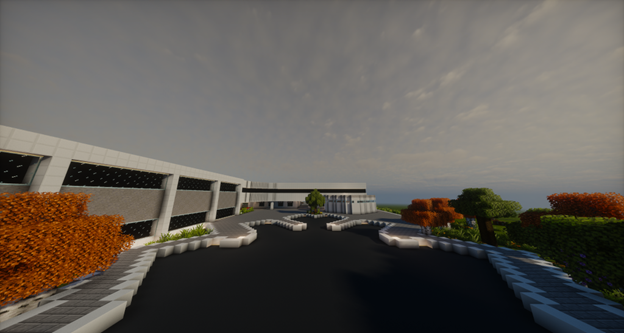
\includegraphics[width=0.9\textwidth]{docs/figuras/Imagem1.png}
    \caption{Réplica virtual do CPTEC/INPE construída no Minecraft.}
    \label{fig:replica_cptec}
\end{figure}

\subsection{Implementação da Realidade Virtual}

A integração do mod Vivecraft permitiu que os participantes explorassem o ambiente virtual em primeira pessoa, aumentando a sensação de imersão no espaço virtual do CPTEC. Essa experiência ampliou o engajamento e facilitou a compreensão dos conceitos científicos incorporados nas missões que compõem a gamificação do ambiente.

\subsection{Desenvolvimento e utilização dos óculos VR artesanais}

O projeto desenvolveu um modelo acessível de óculos de realidade virtual confeccionados com materiais recicláveis, como papelão, elásticos e lentes plásticas reaproveitadas. Este design visa estimular a criatividade, incentivar práticas sustentáveis e ampliar a inclusão tecnológica entre os jovens participantes. Materiais e etapas de montagem foram cuidadosamente planejados e documentados para facilitar sua replicação futura, incluindo a criação de manuais ilustrados.


\begin{figure}[H]
    \centering
    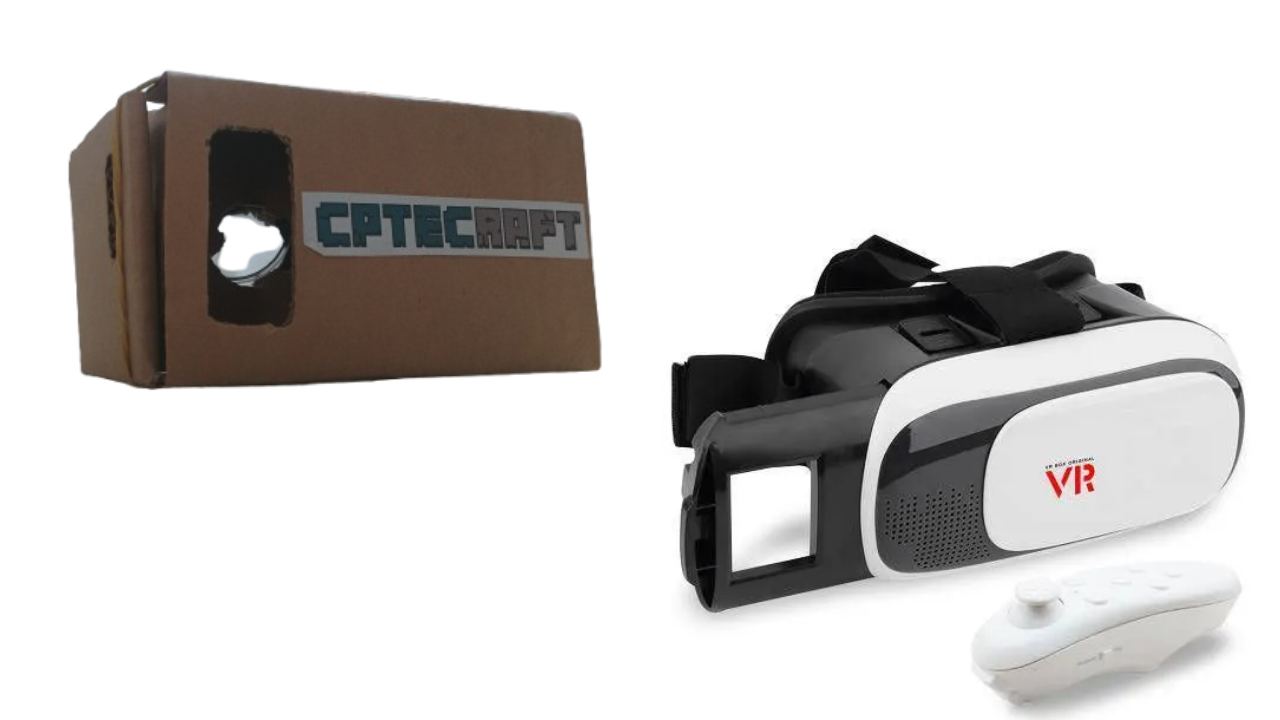
\includegraphics[width=0.5\textwidth]{docs/figuras/Imagem2.png}
    \caption{Óculos VR confeccionados artesanalmente com materiais recicláveis.}
    \label{fig:oculos_vr}
\end{figure}

A implementação prática da confecção destes óculos será realizada nas oficinas educativas previstas para a próxima etapa do projeto, ocasião em que os jovens poderão ser guiados na montagem dos dispositivos, promovendo uma experiência prática e interdisciplinar.

\subsection{Gamificação aplicada ao ensino}

As atividades planejadas envolvem missões e desafios gamificados que exigem aplicação de conceitos de meteorologia, engenharia e sustentabilidade para avançar em objetivos virtuais dentro do ambiente CPTECRAFT. Essa metodologia visa aumentar o engajamento e a motivação pelo aprendizado, associando a interatividade e a diversão a temas científicos relevantes.

Essas oficinas e dinâmicas ainda estão por ser implementadas. Após sua realização, espera-se coletar relatos e avaliações dos participantes para aperfeiçoamento contínuo da proposta pedagógica.

\subsection{Eventos científicos e recepção do público}

No III Encontro de Jovens Cientistas, o CPTECRAFT foi apresentado a crianças, adolescentes e educadores, que interagiram com o ambiente virtual, construíram os óculos VR e participaram das dinâmicas. A receptividade foi muito positiva, demonstrando o potencial da iniciativa para ampliações futuras.

\begin{figure}[H]
    \centering
    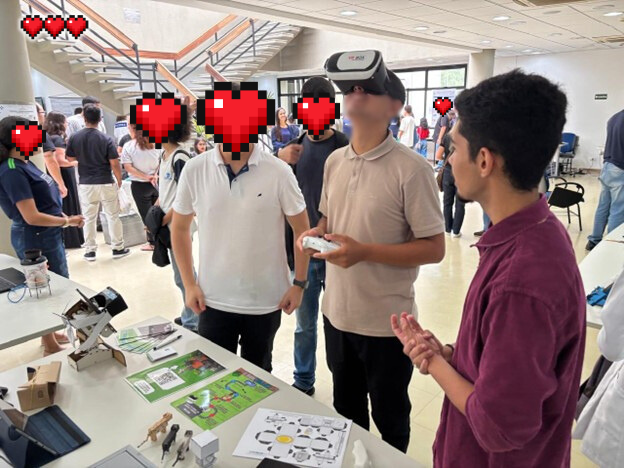
\includegraphics[width=0.6\textwidth]{docs/figuras/Imagem3.png}
    \caption{Participantes interagindo durante o III Encontro de Jovens Cientistas.}
    \label{fig:evento_joes}
\end{figure}

\subsection{Análise quantitativa e qualitativa dos feedbacks}

Para avaliar o impacto do projeto, foi aplicado um questionário utilizando escala Likert de 1 a 5. A Tabela 2.1 mostra os resultados quantitativos das respostas principais.

\begin{table}[!ht]%[htbp] % opções de colocação da tabela no texto
  \begin{center}% use sempre um ambiente para as tabelas
% (opções: center (recomendado), flushright, flushleft)
% NÃO USE \centering com TABELAS se houver \FONTE!
  \caption{Resultados do Questionário (escala de 1 a 5)}
    \begin{tabular}{l|c|c}
\hline % desenha uma linha horizontal
Questão & Média & Desvio Padrão \\
\hline % desenha uma linha horizontal
Motivação para aprender ciência aumentou? & 4,6 & 0,5 \\
Facilidade de uso dos óculos VR? & 4,1 & 0,6 \\
Diversão/engajamento nas atividades? & 4,8 & 0,4 \\
Recomendaria para outros alunos? & 4,7 & 0,5 \\
\hline % desenha uma linha horizontal
    \end{tabular}
  \end{center}
  \FONTE{Dados coletados durante III Encontro de Jovens Cientistas.}
\end{table}

Esses dados indicam alto nível de satisfação e engajamento dos participantes. Comentários espontâneos corroboram as avaliações quantitativas, destacando a experiência prática e o uso da realidade virtual como aspectos muito valorizados:

\begin{itemize}
    \item “Achei muito interessante a possibilidade de poder explorar o CPTEC no Minecraft.”  
    \item “O CPTECRAFT já está disponível ao público?.”  
    \item “Queremos ficar atualizado com os avanços do projeto.”  
\end{itemize}

Em síntese, os resultados quantitativos e qualitativos confirmam a eficácia da metodologia empregada, evidenciando uma aceitação positiva e um alto grau de motivação entre as crianças e adolescentes participantes, consolidando o CPTECRAFT como uma ferramenta promissora para a popularização da ciência e inovação pedagógica.


\section{Discussão dos Resultados}

Os resultados obtidos confirmam a alta aceitação do público e o engajamento gerado pela proposta. Entre os pontos mais valorizados pelos participantes destaca-se a integração entre ciência e jogos digitais, a possibilidade de experiências imersivas com óculos VR de baixo custo e a abordagem gamificada, que transforma conteúdos complexos em desafios interativos e atrativos.

As sugestões coletadas, como a ampliação do acesso a diferentes plataformas, a inserção de jogos educativos e o fortalecimento da divulgação em redes sociais, indicam oportunidades de expansão e melhoria contínua. Essas recomendações reforçam a importância de consolidar o CPTECRAFT como um recurso pedagógico escalável, adaptável a múltiplos contextos escolares e capaz de integrar inovação tecnológica com práticas educativas.

\chapter{Resultados Esperados}

A continuidade do projeto CPTECRAFT espera alcançar resultados expressivos como:  

\begin{itemize}
  \item Ampliar o engajamento de crianças e adolescentes nas áreas STEM por meio de experiências interativas e acessíveis;  
  \item Expandir a utilização da plataforma em escolas públicas e eventos científicos, democratizando o acesso ao ensino inovador;  
  \item Capacitar professores para integrá-lo em suas práticas pedagógicas, promovendo uma formação continuada;  
  \item Desenvolver materiais didáticos e manuais que facilitem a replicação do projeto em diferentes contextos;  
  \item Aperfeiçoar os instrumentos avaliativos para realizar monitoramento constante do impacto educacional;  
  \item Fortalecer parcerias institucionais e captar recursos para assegurar a sustentabilidade e expansão da iniciativa.  
\end{itemize} %% 2o capítulo
%%%%%%%%%%%%%%%%%%%%%%%%%%%%%%%%%%%%%%%%%%%%%%%%%%%%%%%%%%%%%%%%%%%%%%%%%%%%%%%

\chapter{Conclusão}

O projeto CPTECRAFT evidenciou ser uma iniciativa altamente inovadora para a popularização da ciência e o estímulo ao interesse científico entre crianças e adolescentes, combinando tecnologias acessíveis com metodologias lúdicas e gamificadas. A réplica virtual detalhada do CPTEC/INPE foi um ambiente eficaz para aprendizagem ativa e imersiva, suportada pelo uso da realidade virtual com óculos confeccionados de forma sustentável~\citeonline{araujo2016}.

Os resultados obtidos, tanto qualitativos quanto quantitativos, confirmam a aceitação e o potencial transformador da proposta. A identificação de desafios técnicos e pedagógicos aponta para oportunidades importantes de aperfeiçoamento, essenciais para ampliar o alcance e o impacto do projeto.

Com ações previstas de expansão para múltiplas plataformas, melhor suporte técnico e formação docente, o CPTECRAFT se posiciona como um modelo exemplar de inovação educacional, capaz de transformar a forma como a ciência é vivenciada e aprendida pelas novas gerações, fomentando uma sociedade mais informada e tecnologicamente preparada para os desafios do futuro.
\newpage %% 3o capítulo
%\include{./docs/08_04_capitulo4} %% 4o capítulo

%% insira quantos capítulos desejar com o seguinte comando:
%\include{_pasta_do_arquivo_/_meu_arquivo_} %%sem a extensão
%% note que deverá haver um arquivo _meu_arquivo_.tex (com extensão) no diretório _pasta_do_arquivo_

% PARA PUBLICAÇÕES EM INGLÊS:
%% Descomentar essa linha para publicações em inglês
%\bibliographystyle{./template/abnt-alfenglish}

% PARA PUBLICAÇÕES EM PORTUGUÊS:
%% comentar essa linha para publicações em inglês
\bibliographystyle{./template/abnt-alfportuguese}

%% Bibliografia %% não alterar %% obrigatório %testebib
\bibliography{./bib/referencia} %% aponte para seu arquivo de bibliografia no formato bibtex (p.ex: referencia.bib)

%\include{./docs/09_glossario} %% insira os termos do glossário no arquivo glossario.tex %% opcional

\inicioApendice %% opcional, comente esta linha e a seguintes se não houver apendice(s)
%%%%%%%%%%%%%%%%%%%%%%%%%%%%%%%%%%%%%%%%%%%%%%%%%%%%%%%
%Apêndice A
\hypertarget{estilo:apendice}{} %% uso para este Guia
%Este apêndice foi criado apenas para indicar como construir um apêndice no estilo, não existia no original da tese.
%%%%%%%%%%%%%%%%%%%%%%%%%%%%%%%%%%%%%%%%%%%%%%%%%%%%%%
\renewcommand{\thechapter}{}%
\chapter{APÊNDICE A - AUTORIZAÇÃO PARA PUBLICAÇÃO}	% trocar A por B na próxima apêndice e etc
\label{apendiceA}	% trocar A por B na próxima apêndice e etc
\renewcommand{\thechapter}{A}%		% trocar A por B na próxima apêndice e etc

Há dois formulários de autorização para publicação, um para publicações de trabalhos acadêmicos e outro para publicações técnico-científicas, neste apêndice encontram-se os modelos dos formulários e suas respectivas instruções de preenchimento. 

\section{Autorização para Publicação de Trabalho Acadêmico - INPE-393}

\label{instr393}

	\begin{figure}[!ht]
		\caption{Formulário Autorização para Publicação de Trabalho Acadêmico INPE-393.}
		\vspace{6mm}	% acrescentar o espaçamento vertical apropriado entre o título e a borda superior da figura
		\centering
   		\includegraphics[height=16cm]{docs/figuras/form393.png}	   
 		\label{form393}
	\end{figure}


\subsection{Instruções do Formulário INPE-393} 

\begin{enumerate} 

 \item \textbf{série:} com este número o SID identifica as publicações do INPE, composto da sigla da Instituição, número sequencial geral da publicação, sigla e número sequencial do tipo de publicação, exemplo: INPE-14209-TDI/1110;
 
 \item \textbf{número:} será composto da sigla da unidade do SID, mais 4 (quatro) dígitos e do ano em curso. Este número de referência é de controle da unidade emissora. Ex.: SID-0001/2007;

 \item \textbf{título da publicação:} deve ser completo, evitando-se abreviar palavras;

 \item \textbf{nome do autor e do orientador:} estes campos devem ser preenchidos por extenso, da mesma forma em que irão constar da publicação;

 \item \textbf{origem da publicação:} sigla da unidade do servidor (autor da publicação), conforme TQ-001;

 \item \textbf{curso:} sigla do curso, de acordo com a Estrutura de Divisão de Trabalho - EDT do INPE;
 
 \item \textbf{tipo:} assinalar se é tese ou dissertação;

 \item \textbf{apresentação:} colocar a data de aprovação final;

 \item \textbf{revisão técnica:} o responsável designado pela Banca Examinadora para verificação de correções e, na ausência desse, o orientador da tese ou dissertação deve
carimbar, datar e assinar após a versão \emph{on line} do trabalho;

 \item \textbf{revisão de linguagem:} o responsável designado pela Banca Examinadora para verificação de correções, e na ausência deste o orientador deve assinalar a solicitação ou a dispensa da revisão de linguagem e, carimbar, datar e assinar; o revisor deve datar e assinar após a revisão;
 
 \item \textbf{distribuição:} O SID deve informar a quantidade de CD's e de cópias impressas da tese ou dissertação, conforme lista de distribuição;
 
 \item \textbf{verificação de normalização:}  Após a verificação da versão \emph{on line} do trabalho quanto às normas editoriais, o SID deve datar e assinar;
 
 \item \textbf{autorização final:} data e assinatura do Titular de Nível A, conforme TQ-001, a que o Serviço de Pós-Graduação estiver subordinado.
 
 \item \textbf{observações:} para outras informações necessárias. 

\end{enumerate}

\section{Autorização para Publicação - INPE-106}
\begin{figure}[!ht]
	\caption{Formulário Autorização para Publicação de Trabalho Acadêmico INPE-106 folha 1.} 
	\vspace{6mm}	% acrescentar o espaçamento vertical apropriado entre o título e a borda superior da figura
	\centering
	\includegraphics[height=18cm]{docs/figuras/form106.png}
	\label{form106}
\end{figure}

\begin{figure}[!ht]
	\caption{Formulário Autorização para Publicação de Trabalho Acadêmico INPE-106 folha 2.} 
	\vspace{6mm}	% acrescentar o espaçamento vertical apropriado entre o título e a borda superior da figura
	\centering
	\includegraphics[height=18cm]{docs/figuras/form106folha2.png}
	\label{form106a}
\end{figure}

\clearpage
\subsection{Instruções do Formulário INPE-106} 
\label{instr106}


\begin{enumerate}

 \item \textbf{série:} com este número o SID identifica as publicações do INPE, composto da sigla da Instituição, número sequencial geral da publicação, sigla e número sequencial do tipo de publicação, exemplo: INPE-5616-RPQ/671. 
 
 \item \textbf{número:} será composto da sigla da unidade constante da Estrutura Organizacional do INPE (TQ-001), mais 4 (quatro) dígitos e do ano em curso. Este número de referência é de controle da unidade solicitante. Ex: CEA-0001/2007;
 
 \item \textbf{título da publicação:} deve ser completo, evitando-se abreviar palavras;

 \item \textbf{nome do autor, tradutor e editor:}  estes campos devem ser preenchidos por extenso, da mesma forma em que irão constar da publicação;

 \item \textbf{origem da publicação:} sigla da unidade do servidor (autor da publicação), conforme TQ-001;

 \item \textbf{projeto:} sigla do projeto de acordo com a Estrutura de Divisão de Trabalho - EDT do INPE;

 \item \textbf{tipo de publicação:} assinalar o tipo de publicação proposta:

 \begin{enumerate}
  \item{Relátorio de Pesquisa (RPQ)},
  \item{Notas Técnico-Científicas (NTC)},
  \item{Propostas e Relatórios de de Projeto (PRP)},
  \item{Manuais Técnicos (MAN)},
  \item{Publicações Didáticas (PUD)},
  \item{Trabalhos Acadêmicos Externos (TAE)}.
 \end{enumerate}

 \item \textbf{divulgação:} assinalar, de acordo com os critérios de classificação. Se houver Lista de Divulgação, nesta deverá constar os nomes e endereços completos;

 \item \textbf{convênio:} descrever o nome da instituição, quando a publicação for realizada pelo INPE e outra organização, preencher somente para o tipo PRP; 
 
    \item \textbf{autorização preliminar:} data, carimbo e assinatura do Titular da Unidade a que o autor esteja subordinado e, assinatura do revisor que efetuou a revisão técnica aprovando a versão \emph{on line} do trabalho e do revisor que realizou a revisão de linguagem, quando solicitadas; 
    
  \item \textbf{verificação de normalização:} o SID deve datar e assinar após a revisão da adequação às normas editoriais;   
  
  \item \textbf{distribuição:} O SID deve informar a quantidade de CD's e de cópias impressas que deverão ser gravados conforme lista de distribuição;
  
 \item \textbf{autorização final:} data, carimbo e assinatura do Titular de Nível "A", conforme TQ-001, a que o autor da publicação estiver subordinado;
 
 \item \textbf{observações:} para outras informações necessárias, inclusive para descrever as justificativas de uma publicação.
\end{enumerate} %% insira apendices tal qual capítulos acima

%\inicioAnexo
%%%%%%%%%%%%%%%%%%%%%%%%%%%%%%%%%%%%%%%%%%%%%%%%%%%%%%%
%Anexo
%Este anexo foi incluido para explicar como incluir um anexo no estilo, não existia no original desta tese.
%%%%%%%%%%%%%%%%%%%%%%%%%%%%%%%%%%%%%%%%%%%%%%%%%%%%%%%%%%%%%%%%%%%%%%%%%%%%%%%%%
\renewcommand{\thechapter}{}%
\chapter{ANEXO A - ABREVIATURA DOS MESES} %% Título do anexo sempre em maiúsculas. Trocar A por B no próximo anexo e etc
\label{anexoA} %% Rótulo aplicado caso queira referir-se a este tópico em qualquer lugar do texto. Trocar A por B no próximo anexo e etc
\renewcommand{\thechapter}{A}%		% trocar A por B no próximo anexo e etc

\begin{table}[!ht]
 \label{tab:abreviaturas}
  \begin{center}
 	\begin{tabular}{lll}
	 \hline
	  \textbf{Português}    & \textbf{Espanhol}  & \textbf{Italiano}\\ 
   \hline
       janeiro   = jan.   & enero = ene.       & gennaio = gen.\\
       fevereiro = fev.   & febrero = feb.     & febbraio = feb.\\
       março     = mar.   & marzo = mar.       & marzo = mar.\\
       abril     = abr.   & abril = abr.       & aprile = apr.\\
       maio      = maio   & mayo = mayo        & maggio = mag.\\ 
       junho     = jun.   & junio = jun.       & giugno = giu.\\ 
       julho     = jul.   & julio = jul.       & luglio = lug.\\
       agosto    = ago.   & agosto = ago.      & agosto = ago.\\
       setembro  = set.   & septiembre = sep.  & settembre = set.\\
       outubro   = out.   & octubre = oct.     & ottobre = ott.\\
       novembro  = nov.   & noviembre =nov.    & novembre = nov.\\
       dezembro  = dez.   & diciembre = dic.   & dicembre = dic.\\ 
     \hline
   \textbf{Francês}       & \textbf{Inglês}    & \textbf{Alemão}\\
     \hline
       janvier = jan.     & January = Jan.     & Januar = Jan.\\
       février = fév.     & February = Feb.    & Februar = Feb.\\
       mars = mars        & March = Mar.       & März = März\\
       avril = avr.       & April = Apr.       & April = Apr.\\
       mai = mai          & May = May          & Mai = Mai.\\
       juin = juin        & June = June        & Juni = Juni\\
       juillet = juil.    & July = July        & Juli = Juli\\
       août = août        & August = Aug.      & August = Aug.\\
       septembre = sept.  & September = Sept.  & September = Sept.\\
       octobre = oct.     & October = Oct.     & Oktober = Okt.\\
       novembre = nov.    & November = Nov.    & November = Nov.\\
       décembre = déc.    & December = Dec.    & Dezember = Dez. \\ 
    \hline
   \end{tabular}
   \end{center}
	 \FONTE{Adaptada de \citeonline[p.~22]{NBR6023:2002b}.}
\end{table}
%\include{./docs/11_02_anexo2}
%%%%%%%%%%%%%%%%%%%%%%%%%%%%%%%%%%%%%%%%%%%%%%%%%%%%%%%
%Anexo
%Este anexo foi incluido para explicar como incluir um anexo no estilo, não existia no original desta tese.
%%%%%%%%%%%%%%%%%%%%%%%%%%%%%%%%%%%%%%%%%%%%%%%%%%%%%%%%%%%%%%%%%%%%%%%%%%%%%%%%%
\renewcommand{\thechapter}{}%
\chapter{ANEXO C - TIPOS DE REFERÊNCIAS NO \LaTeX} %% Título do anexo sempre em maiúsculas.
\label{anexoC} %% Rótulo aplicado caso queira referir-se a este tópico em qualquer lugar do texto.
\renewcommand{\thechapter}{C}%

\begin{verbatim}

@BOOK{aacr2004, 
  title = {Cataloga{\c{c}}{\~a}o de recursos bibliogr{\'a}ficos 
  pelo {AACR2R} 2002}, 
  edition = {2},
  address = {Bras{\'i}lia},
  publisher = {Editora do Autor},
  author = {Antonia Motta Castro Memória Ribeiro},
  year = {2004}, 
  note = {v{\'a}rias p{\'a}gina{\c{c}}{\~o}es},
 }

@BOOK{rey93,
  title = {Planejar e redigir trabalhos cient\'ificos},
	subtitle = {teste de subtítulo},
  publisher = {Edgard Blücher},
  year = {1993},
  author = {Rey, L.},
  address = {S\~ao Paulo},
  pages = {318},
} 

@MISC{adobe00,
  title = {Adobe Acrobat 5.0.},
  year = {2000},
  note = {1 CD-ROM},
  address = {San Jose, CA},
  publisher = {Adobe Systems},
}


@ARTICLE{amaral98,
  author = {J. R. Amaral},
  title = {{INPE} estuda queda de meteorito na {A}maz{\^o}nia},
  journal = {Jornal Valeparaibano},
  year = {1998},
  month = {22 mar.},
  note = {Caderno 1, p. 12},
  address = {S{\~a}o Jos{\'e} dos Campos},}
}

@BOOK{assireu03,
  title = {Aplica{\c{c}}{\~a}o do operador de fragmenta{\c{c}}{\~a}o  
  assim{\'e}trica {(FA)} na caracteriza{\c{c}}{\~a}o de controles 
  geomorfol{\'o}gicos em reservat{\'o}rios hidrel{\'e}tricos},
  publisher = {INPE},
  year = {2003},
  author = {A. T. Assireu and E. M. L. M. Novo and J. A. Lorenzzetti 
  and C. Z.	F. Braga and I. B. T. Lima and J. L. Stech},
  address = {S{\~a}o Jos{\'e} dos Campos},
  note = {(INPE-9543-RPQ/737)},
  pages = {34},
}

@BOOK{assireu03e,
  title = {Aplica{\c{c}}{\~a}o do operador de fragmenta{\c{c}}{\~a}o 
  assim{\'e}trica {(FA)} na caracteriza{\c{c}}{\~a}o de controles 
  geomorfol{\'o}gicos em reservat{\'o}rios hidrel{\'e}tricos},
  publisher = {INPE},
  year = {2003},
  author = {A. T. Assireu and E. M. L. M. Novo and J. A. Lorenzzetti 
  and C. Z.	F. Braga and I. B. T. Lima and J. L. Stech},
  address = {S{\~a}o Jos{\'e} dos Campos},
  note = {(INPE-9543-RPQ/737)},
  pages = {34},
  url = {goto-/bol.com.br/mirian_cris/2003/01.31.11.23},
  urlaccessdate = {03 maio 2004},
}

@INCOLLECTION{aurelio86, 
  author = {Especializa{\c{c}}{\~a}o},
  editor = {Aur{\'e}lio Buarque Holanda Ferreira},  
  title = {Novo dicion{\'a}rio da l{\'\i}ngua portuguesa},
  publisher = {Nova Fronteira},
  year = {1986},
  address = {Rio de Janeiro}, 
  pages = {698},
  edition = {2},
}

@MANUAL{banon98,
  title = {Apresenta{\c{c}}{\~a}o e ilustra{\c{c}}{\~a}o de 
  uso de uma biblioteca digital},
  author = {G. F. Banon},
  address = {S{\~a}o Jos{\'e} dos Campos},
  year = {1998},
  note = {Palestra realizada no Instituto Nacional de Pesquisas 
  Espaciais (INPE),
	em 17 fev. 1998},
}

@MISC{barbosa70, 
  author = {O. Barbosa},
  title = {Projeto Leste do Tocantins/Oeste do Rio S{\~a}o Francisco},  
  publisher = {Companhia de Pesquisas de Recursos Minerais (CPRM)/
  Departamento Nacional de Produ{\c{c}}{\~a}o Mineral (DNPM)/(PROSPEC)},
  year = {1970},
  address = {Rio de Janeiro}, 
  pages = {170},
  note = {Conv{\^e}nio},
}

@THESIS{boggione03,
  address = {S{\~a}o Jos{\'e} dos Campos},
  author = {G. A. Boggione}, 
  note = {(INPE-10462-TDI/929)},
  pages = {2003. 160},
  school = {Instituto Nacional de Pesquisas Espaciais (INPE)},
  title = {Restaura{\c{c}}{\~a}o de imagens do sat{\'e}lite Landsat-7},
  type = {Disserta{\c{c}}{\~a}o (Mestrado em Sensoriamento Remoto)},
  year = {2003},
}

@ARTICLE{brasil74,
  title = {Decreto-lei nº 6129, de 6 de novembro de 1974. Disp\~oe 
  sobre a transforma{\c{c}}{\~a}o do Conselho Nacional de 
  Desenvolvimento Cient\'ifico e Tecnol\'ogico -- {CNPq}},
  journal = {Lex},
  year = {1974},
  volume = {38},
  pages = {1017-1018},
  month = {out./dez.},
  organization = {Brasil},
  section = {Legisla{\c{c}}{\~a}o Federal e Margin\'alia},
}

@ARTICLE{brasil04,
  title = {Portaria {CCIVIL} nº 388, de 15.04.2004. {D}esigna os 
  membros para compor a {C}omiss\~ao {E}xecutiva do {P}lano de 
  {A}{\c{c}}{\~a}o para a {P}reven{\c{c}}{\~a}o e {C}rontole do 
  {D}esmatamento na {A}maz\^onia {L}egal},
  year = {2004},
  organization = {Brasil},
  url = {http://www.mct.gov.br/legis/portarias/Minist.htm\#2004},
  urlaccessdate = {19 ago. 2004},
}

@MISC{brum99,
  author = {C. G. M. Brum},
  title = {Resistrador anal\'ogico usado para registrar o 
  ru\'ido c\'osmico},
  year = {1999},
  note = {1 fotografia},
  owner = {ePrint},
}

@BOOK{camara01,
  title = {Introdu{\c{c}}{\~a}o {\`a} ci{\^e}ncia da 
  geoinforma{\c{c}}{\~a}o},
  publisher = {INPE},
  year = {2001},
  editor = {G. C\^amara and C. Davis and A. M. V. Monteiro},
  address = {S{\~a}o Jos{\'e} dos Campos},
  pages = {344},
  url = {goto-/sid.inpe.br/sergio/2004/04.22.07.43},
  urlaccessdate = {22 de abr. 2004},
}

@BOOKLET{clima02,
  title = {{C}liman\'alise: {B}oletim de {M}onitoramento e 
  {A}n{\'a}lise {C}lim{\'a}tica},
  address = {S{\~a}o Jos{\'e} dos Campos: INPE},
  month = {jan.},
  year = {2002},
  number = {1},
  url = {http://www.cptec.inpe.br/products/climanalise/capa1.html},
  urlaccessdate = {3 maio 2004},
  volume = {17},
}

@BOOK{clima86,
  title = {Climan\'alise: Boletim de Monitoramento e 
  An\'alise Clim\'atica},
  publisher = {INPE},
  year = {1986},
  address = {S\~ao Jos\'e dos Campos},
  note = {Mensal},
}

@BOOKLET{clima96,
  title = {{C}liman\'alise: {B}oletim de {M}onitoramento e 
  {A}n{\'a}lise {C}lim{\'a}tica},
  address = {S{\~a}o Jos{\'e} dos Campos: INPE},
  month = {jan.},
  year = {1996},
  number = {1},
  pages = {53},
  volume = {11},
}

@BOOK{diller93,
  title = {\LaTeX\ by line},
  publisher = {John Wiley \& Sons},
  year = {1993},
  author = {Antoni Diller},
  address = {Chichester, West Sussex},
  isbn = {0-471-93471-2},
  pages = {291},
}

@INPROCEEDINGS{drummond03,
  author = {I. N. Drummond and L. Godo and S. A. Sandri},
  title = {Learning fuzzy systems with similarity relations},
  booktitle = {Proceedings...},
  year = {2003},
  pages = {516--523},
  address = {Istanbul},
  organization = {International Fuzzy Systems Association 
  World Congress},
  publisher = {ICI/IFSA},
  note = {(INPE-10533-PRE/6005)},
  conference-location = {Istanbul, Turkey},
  conference-number = {10},
  conference-year = {2003},
  isbn = {975-518-208-X},
  org-short = {IFSA},
}

@MISC{fepam92,
  title = {Mata {A}tl\^antica no Rio Grande do Sul},
  year = {1992},
  note = {1 Mapa. Escala 1:250.000},
  address = {Porto Alegre},
  org-short = {FEPAM},
  organization = {Funda{\c{c}}{\~a}o Estadual de Prote{\c{c}}{\~a}o 
  Ambiental Henrique Luis Roessler (FEPAM)},
  subtitle = {tombamento da {R}eserva da {B}iosfera},
  url = {http://www.fepam.rs.gov.br/programas/kfw.asp},
  urlaccessdate = {13 fev. 2002},
}

@ARTICLE{ferreira03,
  author = {R. N. Ferreira and T. M. Richenbach and D. L. Herdies 
  and L. M. V. Carvalho},
  title = {Variability of {S}outh {A}merican convective cloud systems and 
  tropospheric circulation during {J}anuary-{M}arch 1998 and 1999},
  journal = {Monthly Weather Review},
  year = {2003},
  volume = {131},
  pages = {961--973},
  number = {5},
  month = {May},
  note = {(INPE-9991-PRE/5551)},
}

@MISC{filme96,
  title = {Space: helping to complete the picture},
  year = {1996},
  note = {1 videocassete (15 min), VHS, son},
  address = {London},
  publisher = {BNSC},
}

@ARTICLE{formaggio01,
  author = {A. R. Formaggio and J. C. N. Epiphanio and M. D. Sim{\~o}es},
  title = {Radarsat backscattering from an agricultural scene},
  journal = {Pesquisa Agropecu{\'a}ria Brasileira},
  address = {Bras\'ilia},
  year = {2001},
  volume = {36},
  pages = {823--830},
  number = {5},
  url = {http://isi3.isiknowledge.com/portal.cgi?DestApp=WOS&Func=Frame},
  urlaccessdate = {3 maio 2004},
}
 
@BOOK{franca2004,
  title = {Manual para normaliza{\c{c}}{\~a}o de publica{\c{c}}{\~o}es 
  t\'ecnico-cient\'ificas},
  publisher = {UFMG},
  year = {2004},
  author = {Fran{\c{c}a} J\'unia Lessa  and  Vasconcellos Ana Cristina 
  and Magalh{\~a}es Maria Helena A. and  Borges Stella Maris},
  pages = {242},
  address = {Belo Horizonte},
}

@MISC{fsosma02a,
  title = {Atlas dos remanescentes florestais da {M}ata {A}tl{\^a}ntica; 
  per{\'i}odo 1995--2000},
  year = {2002a},
  note = {Cont{\'e}m 11 Mapas. (INPE-9694-PRP/238)},
  address = {S{\~a}o Jos{\'e} dos Campos},
  org-short = {FSOSMA},
  organization = {Funda{\c{c}}{\~a}o SOS Mata Atl\^antica 
  (FSOSMA) / 
  Instituto Nacional de Pesquisas	Espaciais (INPE)},
  pages = {47},
}

@MISC{fsosma02b,
  title = {Atlas dos remanescentes florestais da {M}ata 
  {A}tl{\^a}ntica; 
  per{\'i}odo	1995--2000},
  year = {2002b},
  note = {Cont{\'e}m 11 Mapas. (INPE-9694-PRP/238)},
  address = {S{\~a}o Jos{\'e} dos Campos},
  org-short = {FSOSMA},
  organization = {Funda{\c{c}}{\~a}o SOS Mata Atl\^antica 
  (FSOSMA)/ Instituto Nacional de Pesquisas 	Espaciais (INPE)},
  pages = {47},
  url = {goto-/sid.inpe.br/jeferson/2003/06.02.07.45},
  urlaccessdate = {3 maio 2004},
}

@BOOK{ibge93,
  title = {Normas de apresenta{\c{c}}{\~a}o tabular},
  publisher = {IBGE},
  year = {1993},
  address = {Rio de Janeiro},
  edition = {2},
  isbn = {85-240-0471-1},
  org-short = {IBGE},
  organization = {Instituto Brasileiro de Geografia e Estat\'istica
  (IBGE)},
  pages = {62},
}  

@MANUAL{inpe00,
  title = {Laborat{\'o}rio Associado de Combust{\~a}o e 
  Propuls{\~a}o(LCP)},
  organization = {Instituto Nacional de Pesquisas Espaciais 
  (INPE)},
  address = {Cachoeira Paulista},
  publisher = {INPE},
  year = {2000},
  note = {Folder},
  org-short = {INPE},
}

 @MISC{inpe87,
  title = {S{\~a}o Jos{\'e} dos Campos (SP)},
  year = {1987},
  note = {1 Mapa Topogr{\'a}fico. Escala 1:100.000},
  address = {S{\~a}o Jos{\'e} dos Campos},
  org-short = {INPE},
  organization = {Instituto Nacional de Pesquisas Espaciais (INPE)},
  subtitle = {atualiza{\c{c}}{\~a}o do uso da terra. {SF-23-YD-II-1 
  MI-2769/1}},
}


@MISC{inpe89,
  title = {{CBERS}},
  month = {jan.},
  year = {1989},
  note = {28 transpar{\^e}ncias. 25 x 20 cm},
  address = {S\~ao Jos\'e dos Campos},
  org-short = {INPE},
  organization = {Instituto Nacional de Pesquisas Espaciais (INPE)},
  publisher = {INPE},
}

@MISC{inpe95, 
  organization = {Instituto Nacional de Pesquisas Espaciais (INPE)},
  year = {1995},
  title = {Mem{\'o}ria {T}{\'e}cnico-{C}ient{\'i}fica do INPE},
  org-short = {INPE},
  subtitle = {biblioteca digital},
  url = {http://iris.sid.inpe.br:1905/col/sid.inpe.br/banon/2001/
  04.03.15.36.19/doc/mirror.cgi},
  urlaccessdate = {11 maio 2004},
} 
 
@MANUAL{inpedgi03,
  title = {Cat{\'a}logo CBERS 2},
  organization = {Instituto Nacional de Pesquisas Espaciais (INPE)},
  address = {S{\~a}o Jos{\'e} dos Campos},
  year = {2004},
  org-short = {INPE},
  url = {http://www.dgi.inpe.br},
  urlaccessdate = {03 maio 2004},
}

@MISC{inpedgi04,
  title = {Imagem da cidade de S{\~a}o Jos{\'e} dos Campos},
  year = {2004},
  note = {Cachoeira Paulista, 2000. 1 imagem de sat{\'e}lite. CBERS 2 / 
  Sensor 	CCD. 30 jan. 2004. Base 153 / Ponto: 126, Composi{\c{c}}{\~a}o 
  RGB, bandas	4, 3, 2},
  organization = {Instituto Nacional de Pesquisas Espaciais. Divis{\~a}o de 
  Gera{\c {c}}{\~a}o de Imagens (INPE.DGI)},
  org-short = {INPE.DGI},
}

@MISC{inpedgi05,
  title = {Imagem da cidade de S{\~a}o Jos{\'e} dos Campos},
  year = {2004},
  note = {Cachoeira Paulista, 2000. 1 imagem de sat{\'e}lite. CBERS 1 / 
  Sensor CCD -- Composi{\c{c}}{\~a}o RGB, bandas 4, 3, 2, Base 153 / 
  Ponto: 126},
  organization = {Instituto Nacional de Pesquisas Espaciais. 
  {Divis{\~a}o de Gera{\c {c}}{\~a}o de Imagens (INPE-DGI)}},
  org-short = {INPE-DGI},
  url = {http://www.dgi.inpe.br/html/gal-2.htm},
  urlaccessdate = {20 abr. 2004},
}

@PATENT{inpep95,
  organization = {INSTITUTO NACIONAL DE PESQUISAS ESPACIAIS}, 
  howpublished = {Vladimir Jesus Trava-Airoldi and Evaldo Jose Corat 
  and Edson Del Bosco and Marcia Carneiro Valera and Angel Fidel 
  Pi{\~n}a and Victor Baranauskas and N{\'e}lia Ferreira Leite},
  year = {1995},
  title = {Brocas para uso odontol{\'o}gico ou uso correlato de desgaste ou 
  perfura{\c{c}}{\~a}o revestidas com diamante obtido com as t{\'e}cnicas 
  qu{\'í}micas de crescimento a partir da Fase 
  Vapor-CVD (Chemical Vapor Deposition)},
  note = {21 fev. 1995, 8 out. 2002},
  number = {BR, n. PI 9500865-9},
}

@PATENT {Scha84
  organization = {Santrade Limited},
  year = {1985},
  furtherresp = {Schachner H.},
  title = {Body with superhard coating},
  number = {4,734,339},
  howpublished = {Mar. 29, 1988 and Jun. 24, 1985},
}

@MISC{gomes98,
  title = {Elei{\c{c}}{\~a}o}, 
  year = {1998},
  note = {Entrevistador: M{\'a}rcio Manzi Alvarenga. 
  Uberl{\^a}ndia: Funda{\c{c}}{\~a}o R{\'a}dio e Televis{\~a}o 
  Educativa de Uberl{\^a}ndia, 30 mar. 1998. Entrevista 
  concedida ao programa de televisão "Acontece o seguinte".},
  author = {C Gomes}, 
  subtitle = {poss{\'i}vel candidatura},
}

@BOOK{goossens94,
  title = {The \LaTeX\ companion},
  publisher = {Addison-Wesley},
  year = {1994},
  author = {Michel Goossens and Frank Mittelbach and 
  Alexander Samarin},
  address = {Reading, Massachusetts},
  bibliograpy = {yes},
  index = {yes},
  isbn = {0-201-54199-8},
  pages = {530},
}

@ARTICLE{jeon92,
  author = {B. Jeon and D. A. Landgrebe},
  title = {Classification with spatio-temporal interpixel 
  class dependency 
  contexts},
  journal = {IEEE Transactions on Geoscience and Remote 
  Sensing},
  year = {1992},
  volume = {30},
  pages = {664-672},
  number = {4},
  month = {July},
  note = {Special issue on the 1991 International 
  Geoscience and Remote 
  Sensing
	Symposium (IGARSS'91)},
}

@ARTICLE{jereissati98,
  author = {T. Jereissati},
  title = {Cuidado com o já ganhou},
  journal = {Veja},
  year = {1998},
  address = {S{\~a}o Paulo},
  volume = {31}, 
  pages = {9--11},
  number = {11},
  month =  mar,
  note = {Entrevista concedida a Ernesto Bernardes},
}

@UNPUBLISHED{kishore,
  author = {Ram Kishore and A. K. Mishra},
  year = {},
  title = {Algebra of orthofermions and equivalence of their 
thermodynamics to the infinite U Hubbard model},
  note  = {Aceito pela revista Physica B. 
  Acesso em: 21 jun. 2006.},
}   
        
@INCOLLECTION{kirchhoff91,
  author = {V. W. J. H. Kirchhoff},
  title = {Composi{\c{c}}{\~a}o, estrutura, 
  press{\~a}o e densidade},
  booktitle = {Introdu{\c{c}}{\~a}o {\`a} 
  geof{\'\i}sica espacial},
  publisher = {INPE},
  year = {2001},
  editor = {V. W. J. H. Kirchhoff},
  chapter = {3},
  pages = {31--42},
  address = {S{\~a}o Paulo},
  note = {149 p.},
}

@BOOK{kotait81,
  title = {Editora{\c{c}}{\~a}o cient{\'i}fica},
  publisher = {{\'A}tica},
  year = {1981},
  author = {Ivani Kotait},
  address = {S\~ao Paulo},
  pages = {118},
}

@MANUAL{man90,
  title = {Manual de normas para publica{\c{c}}{\~o}es 
  t{\'e}cnico-cient{\'i}ficas},
  organization = {Instituto Nacional de Pesquisas 
  Espaciais (INPE)},
  org-short = {INPE},
  address = {S{\~a}o Jos{\'e} dos Campos},
  publisher = {INPE},
  year = {1990},
  pages = {133},
  note = {(INPE-5116-MAN/001)},
}

@BOOK{massago04, 
  title = {Um Curso de latex via exemplos},
  publisher = {UFSCAR}, 
  year = {2002},
  author = {Sadao Massago},
  address = {S{\~a}o Paulo},
  url = {http://www2.dm.ufscar.br/~sadao/curso/latex/},
  urlaccessdate = {25 maio 2006},
}


@INCOLLECTION{medeiros01,
  author = {J. S. Medeiros and G. C{\^a}mara},
  title = {Geoprocessamento para projetos ambientais},
  booktitle = {Introdu{\c{c}}{\~a}o {\`a} ci{\^e}ncia da 
  geoinforma{\c{c}}{\~a}o},
  publisher = {INPE},
  year = {2001},
  editor = {G. C\^amara and C. Davis and A. M. V. Monteiro},
  address = {S{\~a}o Jos{\'e} dos Campos},
  note = {(INPE-8568-PRE/4312)},
  url = {goto-/sid.inpe.br/sergio/2004/04.19.15.08},
  urlaccessdate = {23 abr. 2004},
}

@MANUAL{NBR6021:1994a,
  title = {{NBR} 6021},
  organization = {Associa{\c{c}}{\~a}o Brasileira de 
  Normas T{\'e}cnicas (ABNT)},
  address = {Rio de Janeiro},
  month = oct,
  year = {1994a},
  org-short = {ABNT},
  pages = {3},
  subtitle = {Apresenta{\c{c}}{\~a}o de peri\'odicos},
}

@MANUAL{NBR6022:1994b,
  title = {{NBR} 6022},
  organization = {Associa{\c{c}}{\~a}o Brasileira de 
  Normas T{\'e}cnicas (ABNT)},
  address = {Rio de Janeiro},
  month = aug,
  year = {1994b},
  org-short = {ABNT},
  pages = {2},
  subtitle = {Apresenta{\c{c}}{\~a}o de artigos em 
  publica{\c{c}{\~o}es} 
  peri\'odicas},
}

@MANUAL{NBR6023:2002b,
  title = {{NBR} 6023},
  organization = {Associa{\c{c}}{\~a}o Brasileira de Normas 
  T{\'e}cnicas (ABNT)},
  address = {Rio de Janeiro},
  month = aug,
  year = {2002b},
  org-short = {ABNT},
  pages = {24},
  subtitle = {Informa{\c{c}}{\~a}o e documenta{\c{c}}{\~a}o: 
  refer\^encias: 
  elabora{\c{c}}{\~a}o},
}

@MANUAL{NBR6024:1989c,
  title = {{NBR} 6024},
  organization = {Associa{\c{c}}{\~a}o Brasileira de 
  Normas T{\'e}cnicas (ABNT)},
  address = {Rio de Janeiro},
  month = aug,
  year = {1989c},
  org-short = {ABNT},
  pages = {2},
  subtitle = {Numera{\c{c}}{\~a}o progressiva das 
  se{\c{c}}{\~o}es de um documento},  
} 

@MANUAL{NBR6026:1994c,
  title = {{NBR} 6026},
  organization = {Associa{\c{c}}{\~a}o Brasileira de 
  Normas T{\'e}cnicas (ABNT)},
  address = {Rio de Janeiro},
  month = mar,
  year = {1994c},
  org-short = {ABNT},
  pages = {2},
  subtitle = {Legenda bibliogr{\'a}fica},
}

@MANUAL{NBR6027:1989b,
  title = {{NBR} 6027},
  organization = {Associa{\c{c}}{\~a}o Brasileira de 
  Normas T{\'e}cnicas (ABNT)},
  address = {Rio de Janeiro},
  month = aug,
  year = {1989b},
  org-short = {ABNT},
  pages = {2},
  subtitle = {Sum{\'a}rio},
}

@MANUAL{NBR6028:1990,
  title = {{NBR} 6028},
  organization = {Associa{\c{c}}{\~a}o Brasileira de 
  Normas T{\'e}cnicas (ABNT)},
  address = {Rio de Janeiro},
  month = may,
  year = {1990},
  org-short = {ABNT},
  pages = {3},
  subtitle = {Resumos},
}

@MANUAL{NBR6029:2005b,
  title = {{NBR} 6029},
  organization = {Associa{\c{c}}{\~a}o Brasileira de 
  Normas T{\'e}cnicas (ABNT)},
  address = {Rio de Janeiro},
  month = sep,
  year = {2005b},
  org-short = {ABNT},
  pages = {9},
  subtitle = {Informa{\c{c}}{\~a}o e documenta{\c{c}}{\~a}o: 
  livros e folhetos: 
  Apresenta{\c{c}}{\~a}o},
}

@MANUAL{NBR6032:1989,
  title = {{NBR} 6032},
  organization = {Associa{\c{c}}{\~a}o Brasileira de 
  Normas T{\'e}cnicas (ABNT)},
  address = {Rio de Janeiro},
  month = aug,
  year = {1989},
  org-short = {ABNT},
  pages = {14},
  subtitle = {Abrevia{\c{c}}{\~o}es de T{\'i}tulos de 
  peri{\'o}dicos e 
  publica{\c{c}}{\~o}es 
  seriadas},
}

@MANUAL{NBR6033:1989,
  title = {{NBR} 6033},
  organization = {Associa{\c{c}}{\~a}o Brasileira de 
  Normas T{\'e}cnicas (ABNT)},
  address = {Rio de Janeiro},
  month = aug,
  year = {1989},
  org-short = {ABNT},
  pages = {5},
  subtitle = {Ordem alfab{\'e}tica},
}

@MANUAL{NBR6034:1989d,
  title = {{NBR} 6034},
  organization = {Associa{\c{c}}{\~a}o Brasileira de 
  Normas T{\'e}cnicas (ABNT)},
  address = {Rio de Janeiro},
  month = aug,
  year = {1989d},
  org-short = {ABNT},
  pages = {3},
  subtitle = {Prepara{\c{c}}{\~a}o de {\'i}ndice de publica{\c{c}}{\~o}es},
}

@MANUAL{NBR10520:2002a,
  title = {{NBR} 10520},
  organization = {Associa{\c{c}}{\~a}o Brasileira de 
  Normas T{\'e}cnicas (ABNT)},
  address = {Rio de Janeiro},
  month = aug,
  year = {2002a},
  org-short = {ABNT},
  pages = {7},
  subtitle = {Informa{\c{c}}{\~a}o e documenta{\c{c}}{\~a}o: 
  apresenta{\c{c}}{\~a}o de 
  cita{\c{c}}{\~o}es em documentos},
}

@MANUAL{NBR10521:1988,
  title = {{NBR} 10521},
  organization = {Associa{\c{c}}{\~a}o Brasileira de 
  Normas T{\'e}cnicas (ABNT)},
  address = {Rio de Janeiro},
  month = oct,
  year = {1988},
  org-short = {ABNT},
  pages = {2},
  subtitle = {Numera{\c{c}}{\~a}o internacional para livro: isbn},
}

@MANUAL{NBR10719:1989a,
  title = {{NBR} 10719},
  organization = {Associa{\c{c}}{\~a}o Brasileira de 
  Normas T{\'e}cnicas (ABNT)},
  address = {Rio de Janeiro},
  month = aug,
  org-short = {ABNT},
  pages = {17},
  subtitle = {Apresenta{\c{c}}{\~a}o de relat{\'o}rios  
  t{\'e}cnico-cient{\'i}ficos},
  year = {1989a},
}

@MANUAL{NBR12256:1992,
  title = {{NBR} 12256},
  organization = {Associa{\c{c}}{\~a}o Brasileira de 
  Normas T{\'e}cnicas (ABNT)},
  address = {Rio de Janeiro},
  month = apr,
  year = {1992},
  org-short = {ABNT},
  pages = {4},
  subtitle = {Apresenta{\c{c}}{\~a}o de originais},
}

@MANUAL{NBR14724:2005a,
  title = {{NBR} 14724},
  organization = {Associa{\c{c}}{\~a}o Brasileira de 
  Normas T{\'e}cnicas (ABNT)},
  address = {Rio de Janeiro},
  month = jan,
  year = {2005a},
  org-short = {ABNT},
  pages = {9},
  subtitle = {Informa{\c{c}}{\~a}o e documenta{\c{c}}{\~a}o: 
  trabalhos acad{\^e}micos: apresenta{\c{c}}{\~a}o},
}

@TECHREPORT{mauri:2003,
   author = {Instituto Nacional de Pesquisas (INPE)}, 
   year = {2003},
   title = {Resolu{\c{c}}{\~a}o do problema de programa{\c{c}}{\~a}o 
   de tripula{\c{c}}{\~o}es de um sistema de transporte p{\'u}blico via 
   simulated annealing},
   address = {Ouro Preto},
   organization = {Departamento de Ci{\^e}ncia da Computa{\c{c}}{\~a}o{-} 
   Universidade Federal de Ouro Preto},
   url = {http://www.decom.ufop.br/prof/marcone/Orientacoes/
   PPTviaSimulatedAnnealing.pdf},
   urlaccessdate  = {28 ago. 2006},   
   note = { 98p. Relat{\'orio t{\'e}cnico}},
}


@THESIS{padua04,
  address = {S{\~a}o Jos{\'e} dos Campos},
  author = {Marcelo Banik  P\'adua},
  pages = {2004. 162},
  note = {(INPE-12565-TDI/1004)},
  school = {Instituto Nacional de Pesquisas Espaciais (INPE)},
  title = {Estudo da indu{\c{c}}{\~a}o eletromagn{\'e}tica na 
  caracteriza{\c{c}}{\~a}o de estruturas profundas sob a borda sul do
  cr{\'a}ton de S{\~a}o Francisco},
  type = {Tese (Doutorado em Geof{\'i}sica)},
  url = {http://mtc-m16.sid.inpe.br:80/rep/sid.inpe.br/jeferson/
  2005/02.15.14.39},
  urlaccessdate = {22 ago. 2005}, 
  year = {2004},
}

@MISC{padua05,
  author = {Irani In{\'a}cio Cordeiro P\'adua},
  title = {Estilo TDIINPE LaTeX},
  year = {2005},
  note = {58 transparências}, 
  address = {S{\~a}o Jos{\'e} dos Campos},
  publisher = {INPE},
  subtitle = {Curso de editora{\c{c}}{\~a}o eletr{\^o}nica e 
publica{\c{c}}{\~a}o t{\'e}cnico-cient{\'i}fica},
  url = {http://ePrint.sid.inpe.br:1905/rep/sid.inpe.br/ePrint@1905/
  2005/10.26.13.54},
  urlaccessdate = {19 jun. 2006},
}

@MISC{parc96, 
  title = {Parc-nov.xls},
  organization = {Instituto Nacional de Pesquisas Espaciais (INPE)},
  address = {S{\~a}o Jos{\'e} dos Campos},
  year = {1996},
  note = {tabela de par{\^a}metros dendrom{\'e}tricos para estimativa de 
  biomassa.  1 disquete. 
  3.5 pol. 120832 caracteres. Excel.},
}

@BOOK{prado01,
  title = {Trajet{\'o}rias espaciais e manobras assistidas por gravidade},
  publisher = {INPE},
  year = {2001},
  author = {F. A. B. A. Prado},
  address = {S{\~a}o Jos{\'e} dos Campos},
  pages = {169},
}

@MISC{radam83,
  title = {Folhas {SC}. 24/25 Aracaj{\'u}/Sergipe}, 
  subtitle = {geologia, geomorfologia, pedologia, vegeta{\c{c}}{\~a}o e 
  uso potencial da terra}, 
  year = {1983},
  organization = {PROJETO RADAMBRASIL},
  address = {Rio de Janeiro},
  publisher = {IBGE},
  note = {5 mapas col. (Levantamento de Recursos Naturais, 30)},
  pages = {856},
 
}

@ARTICLE{raun95,
  author = {W. R. Raun and H. J. Barreto},
  title = {Regional maize grain response to applied phosphorus in 
  {C}entral	{A}merica},
  journal = {Agronomy Journal},
  year = {1995},
  volume = {87},
  pages = {208-213},
  number = {2},
  month = {Mar.},
  note = {Resumo em \textbf{Abstracts in Tropical Agriculture}, v. 20, 
  n. 12, p. 100, Dec. 1995},
}

@MANUAL{rca73,
  title = {Silicon transistor for 200-watt quasi-complementary symmetry 
  audio	amplifiers with parallel output transistor},
  organization = {Radio Corporation of America (RCA)},
  address = {Somerville, NJ},
  year = {1973},
  note = {Cat\'alogo},
  org-short = {RCA},
}

@BOOK{rey93,
  title = {Planejar e redigir trabalhos cient\'ificos},
	publisher = {Edgard Blücher},
  year = {1993},
  author = {Rey, L.},
  address = {S\~ao Paulo},
  pages = {318},
} 
  
@INPROCEEDINGS{rocha2005,
 author = {Elizabeth Rocha  and  Maria Feitosa Barros and Rafael 
 Silva Cruz and Carla Bernadete Madureira},
 title = {Uso de modelos digitais de eleva{\c{c}}{\~a}o de 
imagens de Radar para extra{\c{c}}{\~a}o de fei{\c{c}}{\~o}es 
topogr{\'a}ficas {-}um estudo de caso Maci{\c{c}}o da Tijuca, vertente 
Ba{\'i}a da Guanabara},
 booktitle = {Anais...},
 year = {2005}, 
 pages = {4469--4472}, 
 publisher = {{INPE}}, 
 address = {S{\~a}o Jos{\'e} dos Campos},
 organization = {Simp{\'o}sio Brasileiro de Sensoriamento Remoto},
 conference-location = {Goi{\^a}nia},
 conference-number = {12},
 conference-year = {2005},
 url = {http://marte.dpi.inpe.br:80/rep/ltid.inpe.br/sbsr/2004/
 11.20.11.59},
 urlacessdate = {12 jun. 2006},   
}
 
@MISC{rudorff04,
  author = { B. F. T. Rudorff},
  title = {Autoriza{\c{c}}{\~a}o para c{\'o}pia de publica{\c{c}}{\~a}o},
  year = {2004},
  note = {[mensagem pessoal].Mensagem recebida por \url{pubtc@sid.inpe.br} 
  em 19 abr. 2004},
}

@BOOK{saty04,
  title = {Rudimentos de meteorologia dinâmica},
  publisher = {INPE},
  year = {2004},
  author = {Satyamurty, P.},
  address = {S{\~a}o Jos{\'e} dos Campos},
  isbn = {85-17-00019-6},
  note = {(INPE-11437-RPQ/769)},
  pages = {154},
  url = {http://mtc-m16.sid.inpe.br/rep-/sid.inpe.br/marciana/2004/
  10.07.14.05},
  urlaccessdate = {02 out. 2006},
}

@INPROCEEDINGS{shima03,
  author = {Yosio Edemir Shimabukuro and Tomoaki Miura and Alfredo Huete 
  and  Egidio Arai and Fernando Del Bon Esp\'irito-Santo and Marcelo 
  Lopes Latorre},
  title = {An{\'a}lise dos dados hiperespectrais do {EO}-1 obtidos 
  sobre a {F}loresta {N}acional de {T}apaj{\'o}s no estado do {P}ar{\'a}},
  booktitle = {Anais...},
  year = {2003},
  pages = {1099--1106},
  publisher = {INPE},
  address = {S{\~a}o Jos{\'e} dos Campos},
  organization = {Simp{\'o}sio Brasileiro de Sensoriamento Remoto},
  note = {1 CD-ROM},
  conference-location = {Belo Horizonte},
  conference-number = {11},
  conference-year = {2003},
}

@INPROCEEDINGS{shima03e,
  author = {Yosio Edemir Shimabukuro and Tomoaki Miura and 
  Alfredo Huete and  Egidio Arai and Fernando Del Bon Esp{\'i}rito-Santo 
  and Marcelo Lopes Latorre},
  title = {An{\'a}lise dos dados hiperespectrais do {EO}-1 obtidos 
  sobre a   {F}loresta {N}acional de {T}apaj{\'o}s no estado do {P}ar{\'a}},
  booktitle = {Anais...},
  year = {2003},
  pages = {1099--1106},
  publisher = {INPE},
  address = {S{\~a}o Jos{\'e} dos Campos},
  organization = {Simp{\'o}sio Brasileiro de Sensoriamento Remoto},
  conference-location = {Belo Horizonte},
  conference-number = {11},
  conference-year = {2003},
  url = {goto-/ltid.inpe.br/sbsr/2002/11.17.13.39},
  urlaccessdate = {22 abr. 2004},
}

@INCOLLECTION{souza01,
  author = {M. L. O. Souza},
  title = {Sistemas de controle de atitude e de {\'o}rbita},
  booktitle = {Fundamentos de tecnologia espacial},
  publisher = {INPE},
  year = {2001},
  editor = {A. F. B. A. Prado and H. K. Kuga},
  chapter = {10},
  pages = {133--137},
  address = {S{\~a}o Jos{\'e} dos Campos},
}

@ARTICLE{taylor96,
  author = {D. Taylor},
  title = {{WWW} weatherfax images},
  journal = {{YACHT-L}},
  year = {1996},
  url = {listserv@hearn.bitnet},
  urlaccessdate = {17 Apr. 1996},
}

@BOOK{tierno2006,   
  title = {Ferramentas do word de apoio para utiliza{\c{c}}{\~a}o do 
  TDIINPE.dot},
  publisher = {INPE},  
  year = {2006},  
  author = {Maria Ros{\'a}rio Giffoni Tierno}, 
  address = {S{\~a}o Jos{\'e} dos Campos},   
  pages = {50},  
  url = {http://ePrint.sid.inpe.br:1905/rep/sid.inpe.br/
  ePrint@1905/2006/}, 
  urlaccessdate = {jul. 2006},
}

@MANUAL{tourrilhes2001,
  author = {Jean Tourrilhes},
  year = {2001},
  title = {A bit More about the technologies involved},
  subtitle = {Information and documentation},
  url = {http://www.hpl.hp.com/personal/Jean_Tourrilhes/Linux/Linux.
  Wireless.Overview.html},
  urlaccessdate = {15 jun. 2005},
}

%transparência
 @MISC{traina2002,
  author ={Agma Juici Machado Traina and Traina, Junior, Caetano}
  title = {Como escrever artigos cient{\'i}ficos},
  publisher = {UFSCAR},
  year = {2002},
  note = {27 transparências},
  url = {http://gbdi.icmc.usp.br/disciplinas/sce-5845/ComoEscrever
  /Single.html},
  urlaccessdate = {25 maio 2006},
}

 @INCOLLECTION{venancio84,
  author = {Alberto {VEN{\^A}NCIO FILHO}},
  title =  {Constituição de 1934},
  booktitle = {Dicion{\'a}rio hist{\'o}rico biogr{\'a}fico brasileiro 
  1930-1983},
  editor = {I. Beloch  and  A. A. Abreu},
  publisher = {FGV, CPDOC : FINEP}, 
  year = {1984},
  address = {Rio de Janeiro}, 
  pages = {913-914},
  volume = {2},
}  

@INCOLLECTION{camposvelho97,
  author = {Haroldo Fraga, Campos Velho},
  title =  {Constituição de 1934},
  booktitle = {Dicion{\'a}rio hist{\'o}rico biogr{\'a}fico brasileiro 
  1930-1983},
  editor = {I. Beloch  and  A. A. Abreu},
  publisher = {FGV, CPDOC : FINEP}, 
  year = {1997},
  address = {Rio de Janeiro}, 
  pages = {913-914},
  volume = {2},
}  

%Este é um exemplo de capítulo de livro 

@INCOLLECTION{sousa:2004,
  author = {SOUSA, F.L. and RAMOS, F.M. and GALSKI, R.L. and MURAOKA, I.},
  title = {Generalized extremal optimization: a new meta-heuristic inspired by a model of natural evolution},
  booktitle = {Recent developments in biologically inspired computing},
  publisher = {Idea Group Inc.},
  year = {2004},
  editor = {Leandro N. de Castro and Fernando J. Von Zuben},
  chapter = {},
  pages = {41--60},
  address = {Hershey PA},
}

 @ARTICLE{dias,
 author = {Silva, Dias, M. A. F.},
 title = { Sistemas de Mesoescala e previs{\~a}o de tempo a curto prazo},
 journal = {Revista Brasileira de Meteorologia},
 volume = {2},
 pages = {133-150},
 year = {1987},
}

%Este exemplo segundo uma aluna fica com et al nos autores 

@ARTICLE{Oost02, 
 author = {W.A. Oost and G.J Komen and C.M.J. Jacobs and C.V. Oort},
 title = {New Evidence For a Relation Between Wind Stress and  Wave age 
 from Measurements During Asgamage},
 journal = {Boundary Layer Meteorology},
 year = {2002},
 volume = {103},
 pages = {409-438}
}

%Este é um exemplo de título de tese com subtítulo

@THESIS{leite04,
 address = {Maceió},
 author = {C.C. Leite},
 school = {Universidade Federal de Alagoas (UFAL)},
 title = {Características da {C}amada {L}imite {C}onvectiva durante a 
 transi{\c{c}}{\~a}o da  esta{\c{c}}{\~a}o seca para chuvosa na {A}maz\^onia (2002)},
 subtitle = {{C}omparação {F}loresta/{P}astagem ({DRY TO WET AMC}/{LBA})},
 type = {Dissertação (Mestrado em Meteorologia)},
 year = {2004},
}


%Este é um exemplo de capítulo de livro, onde foi adicionado o campo nota, 
%para indicar a série 

 @INCOLLECTION{athanassoula01,
 author = {Evangelia Athanassoula},
 title = {Secular evolution of disc galaxies and of their components},
 booktitle = {Mapping the galaxy and nearby galaxies},
 publisher = {Springer},
 year = {2008},
 editor = {Keiichi Wada and Françoise Combes},
 address = {New York},
 pages = {47--54},
 note = {Astrophysics and Space Science Proceedings},
}

%Este é um exemplo para decreto publicado em coletânea, 
%criado pelo Estado de São Paulo

 @ARTICLE{saopaulo98,
 organization = {S{\~a}o Paulo {(Estado)}},  
 title = {Decreto nº 42.822, de 20 de janeiro de 1998},
 journal = {Lex:},	
 section = {colet\^anea de legisla{\c{c}}{\~a}o e jurisprud\^encia},
 year = {1998},
 volume = {62},
 number = {3},
 pages = {217-220},
 address = {S{\~a}o Paulo },
}

%Este é um exemplo para título contendo aspas 
 @THESIS{mattos/06,
 address = {S{\~a}o Jos{\'e} dos Campos},
 author = {Mattos, Jo{\~a}o Gerd Zell},
 note = {(INPE-14794-TDI/1237)},
 pages = {2006. 129},
 school = {Instituto Nacional de Pesquisas Espaciais (INPE)},
 title = {Sensibilidade do uso de "Pseudo-temps" na  assimila{\c{c}}{\~a}o 
 de dados do modelo de  circula{\c{c}}{\~a}o geral atmosf{\'e}rica do CPTEC/COLA},
 type = {Tese (Doutorado em Meteorologia)},
 year = {2006},              
 url = {http://urlib.net/sid.inpe.br/mtc-m17@80/2007/02.15.17.37},
 urlaccessdate = {12 abr. 2011},
}
 
%Este é um exemplo de título com fórmulas e sigla
 @ARTICLE{chedin:2003,
 author = {A. Chedin and S. Serrar and N.A. Scott and C. Crevoisier and R. Armante},
 title = {First global measurement of midtropospheric {CO}$_2$ 
         from {NOAA} polar	satellites: tropical zone},
 journal = {J. Geophys. Res.},
 volume = {108 (D18)},
 pages = {13 pp.},
 year =  {2003},
 note =  {4581, doi:10.1029/2003JD003439},
}

%Este é um exemplo de relatório técnico cujo título tem subtítulo e 
% cujo autor é uma entidade

@TECHREPORT{IPCC:2001,
   year = {2001},
   title = {Climate change 2001},
	 subtitle = {the physical science basis. contribution of working group I
	 to the third assessment
   report of the intergovernmental panel on climate change},
   address = {Cambridge, United Kingdom},
   organization = {Intergovernmental Panel on Climate Change (IPCC)},
   url = {http://www.grida.no/publications/other/ipcc_tar/},
   urlaccessdate  = { },  
   note = {98p. Relat{\'orio t{\'e}cnico}},
}

%Este é um exemplo de livro com subtítulo 

@BOOK{Beale:90,
  author = {Beale, R.; Jackson, T.},
  title =   {Neural computing},
	subtitle = {an introduction},
  edition =  {},
  address =  {New York, NY},
  publisher = {Adam Higler Bristol},
  year =  {1990},
}

\end{verbatim}

%\inicioIndice
%\include{./docs/12_contracapa}
\end{document}